\begin{abstract}
%We consider an investor with preferences that accord with Generalized
%Disappointment Aversion. Such an investor cares about downside risk and
%we assume he recognizes the heavy tail feature of asset return
%distributions. We argue that when a market is dominated by rational
%investors of this kind, the return distributions of equities that are
%actively traded in this market must have very similar tail-indices. We
%also show, in contrast, the scale parameters of the return
%distributions may differ hugely from one another.
%On the other hand, whether or not all equities in a multivariate model
%have the same tail-index is a dividing issue for multivariate GARCH
%models proposed in the literature. Therefore, it is important to analyze
%data of real equity returns and see how close to each other the
%tail-indices actually are.
%In this work empirical results are also presented and they appear
%to support the conclusion that the tail-indices are very similar,
%with respect to the confidence bands of estimation.
\end{abstract}

\section{Introduction}\setcounter{equation}{0}
It is one of the stylized facts of financial econometrics that 
returns of speculative prices are {\em heavy-tailed.} There is no agreement
in the literature about how heavy these tails really are. For example, Barndorff-Nielsen and Shephard
\cite{barndorff:shephard:2001} and Eberlein \cite{eberlein:2001} favor ``semi-heavy'' tails
which are comparable with those of a gamma \ds . On the other
hand, tails of returns have been studied in great detail 
in the extreme value community. Among extreme value specialists
there is general agreement that returns $X_t$ have tails of power-law-type, i.e.,
\beam\label{eq:1}
\P(X_t>x)\sim c_+ \,x^{-\alpha_{\rm up}}\quad\mbox{and}\quad \P(X_t<-x)\sim c_-\,x^{-\alpha_{\rm low}}\,,\quad\xto\,,
\eeam  
where $c_{\pm}$, $\alpha_{\rm up}$ and $\alpha_{\rm low}$ are positive constants.\footnote{Here and in what
  follows, $f(x)\sim g(x)$ for positive \fct s $f$ and $g$ means 
that $f(x)/g(x)\to 1$ as $\xto$.} See for example, Embrechts et
al. \cite{embrechts:klueppelberg:mikosch:1997}, Jansen and de Vries
\cite{jansen1991frequency}, Mikosch \cite{mikosch:2003}, Resnick
\cite{resnick:2007}.  
In the extreme value literature it is common to replace the constants $c_\pm$ by suitable
{\em slowly varying} \fct s; cf. Embrechts et
al. \cite{embrechts:klueppelberg:mikosch:1997}, Chapter 3. In this
paper, for the  
sake of argument, we stick to the condition \eqref{eq:1}.
\par
There are some good theoretical reasons for the appearance of power-law tails in situations where certain moments 
of data are believed to be infinite. Tails of type \eqref{eq:1}
describe the maximum domain of attraction of the  
Fr\'echet \ds\ $\Phi_{\alpha_{\rm up}}(x)=\exp(-x^{-\alpha_{\rm up}})$ for $x>0$, i.e., scaled maxima of an iid \seq\ $(X_t)$ with
upper tail described in \eqref{eq:1} converge in \ds\ to $\Phi_{\alpha_{\rm up}}$.
Equivalently, power-law tails are prescribed by the 
generalized Pareto \ds\ which is the limit \ds\ of the excesses of $X_t$ above high thresholds, i.e., for a suitable positive scaling \fct\ $a(u)$,
\beao
\P((X_t-u)/a(u)>x \mid X_t>x) \to (1+ x/\alpha_{\rm up})^{-\alpha_{\rm up}}\,,\qquad u\to\infty\,.
\eeao
The aforementioned results 
are considered very natural for iid and weakly dependent strictly stationary \seq s of random variables $(X_t)$; 
in the world of extremes they are the analogs
of the \clt\ from the world of sums.
\par
In the literature on extremes for return data one finds the 
statement that {\em estimated} values $\hat \alpha_{\rm up}$ and $\hat \alpha_{\rm low}$ 
of the tail-indices $\alpha_{\rm up}$ and $\alpha_{\rm low}$,
respectively, typically have the tendency that $\hat \alpha_{\rm
  up}>\hat \alpha_{\rm low}$. 
This observation is often explained by the fact that investors are
more prone to negative than to positive news in the market. 
Moreover, in the literature the {\em estimated} tail-indices $\hat \alpha$ (both in the left and right tails) 
are typically found in the range $(2,4)$. For an illustration, see
Figure~\ref{fig:1} where estimates $\hat \alpha_{\rm low}$ 
in three sectors of the Standard \& Poors 500 index  are shown. The
estimates are based on 1304 observations of daily return 
data from 4 January 2010 to 31 December 2014.
\par
When looking at Figure~\ref{fig:1} one might ask the following questions:
\begin{itemize}
\item
In view of the wide \asy\ confidence bands for the estimators of tail-indices, 
are the tail-indices from different series really distinct?
\item
Are there some {\em theoretical} reasons supporting the fact that the tail-indices from different series are {\em not} 
distinct?
\end{itemize}
In this paper, we try to find some answers to these questions. 
\par
The estimator of the tail-index $\alpha>0$  in the model
\beao
\P(X_t>x)\sim c\,x^{-\alpha}\,,\qquad \xto\,,
\eeao
favored in the literature  is the {\em Hill estimator}; the graphs in 
Figure~\ref{fig:1} are based on this estimator. We introduce this estimator in Section~\ref{sec:1} and discuss 
some of its virtues and vices. In addition to tail-index estimation we also discuss the related problem of
estimation of the scale parameters in the tail (these are the constants $c_+$ and $c_-$ in \eqref{eq:1}). 
%{\red check} It turns out 
%that the simultaneous estimation of the tail-index and the scale parameter are strongly related.
\par
In Section~\ref{sec:2} we discuss the theoretical problem of appearance of power-law tails in models 
for daily or, more generally, low-frequency
return data. In particular, in Section~\ref{subsec:garch} we address the power-law tails of univariate and multivariate GARCH models as potential models
for a set of return data from distinct assets. As a matter of fact, under mild conditions, the aforementioned models
have power-law tails due to their relation with so-called {\em stochastic recurrence equations}. Moreover, some of the {\em standard} multivariate 
GARCH models as the CCC ensure that the component-wise marginal \ds s have power-law tails with the same index.
\par
In Section~\ref{sec:3} we discuss an economic argument for the fact that return data of similar assets
(such as return series in a given sector of the S\&P 500 index) may have tail-indices which are close to each other.
We argue based on a  utility \fct\ approach. We explicitly recognize the behavioral
concern for downside risk in an investor's evaluation of a portfolio
using the framework of Generalized Disappointment Aversion (GDA)
introduced by Routledge and Zin \cite{routledge2010generalized}. GDA
is an extension of the concept of Disappointment Aversion (DA) of Gul \cite{gul:1991} who derived DA from first principles (axiomatic).

In Section~\ref{sec:4} we summarize the discussion of the previous
sections. 

\section{Power-law tails of return series: some empirical results}\label{sec:1}\setcounter{equation}{0}
In this section, we assume the model \eqref{eq:1} for the tails of the marginal
\ds\ of a univariate return series $(X_t)$. For the sake of argument, we assume
that this series constitutes a strictly stationary \seq . In what follows, we focus
on the left tail of the \ds , i.e., on the losses. 
However, it is common to present the tail-index estimators
for positive data. Therefore we will multiply the losses $X_t$ by
minus one, swapping the negative with the positive values.
For simplicity, we also suppress subscripts in the notation:
\beam\label{eq:1a}
\P(-X_t>x)\sim c\,x^{-\alpha}\,,\qquad \xto\,,
\eeam
where we assume that the two parameters -- the tail-index  $\alpha$ and the scale parameter
$c$ -- are positive. They play crucial roles for the understanding of the risk hidden in the data, hence 
for asset allocation and risk management. These parameters are market characteristics  and provide a simple but 
useful description of the risk, for example in terms of high quantiles such as
Value-at-Risk. Alternatively, these parameters can be
used for model building of the equities in the market such as the GARCH model; see Section~\ref{sec:2}.
%With these motives in mind, we present a survey of the
%tail-indices and scale parameters of 3 sectors, namely ``Energy'',
%``Consumer Staples'' and ``Information Technology'', of the S\&P 500
%index.

\subsection{Hill estimates of lower tail-indices}\label{sec:Hill}
Various estimators of the tail-index $\alpha$  in the model
\eqref{eq:1a} have been proposed in the literature;
see Embrechts et al. \cite{embrechts:klueppelberg:mikosch:1997}, de
Haan and Ferreira \cite{haan:ferreira:2006}, Resnick
\cite{resnick:2007}. The most popular among them was introduced  by
Hill \cite{hill1975simple}.
Given a sample $-X_1,\ldots,-X_n$ whose marginal \ds\ satisfies  \eqref{eq:1a}, calculate
the order statistics $X_{(1)}\le \cdots\le X_{(n)}$  and construct the
{\em Hill estimator}:
\beao%\label{eq:Hill_index}
  \hat \alpha_k = \Big(
    {1 \over k} \sum_{i=1}^k \log {X_{(n-i+1)} \over X_{(n-k)}}
    \Big)^{-1}\,.
\eeao
Here $k$  is the number of upper order statistics in the sample used
for the estimation. The estimator $\hat \alpha_k$ is 
a maximum-likelihood estimator of $\alpha$ based on the $k$ upper
order statistics in the pure Pareto model (recall that 
we multiplied the data by minus one)
\beam\label{eq:3}
\P(-X_t>x)= \dfrac{K^\alpha}{x^\alpha}\,,\qquad x>K\,,
\eeam
under the hypothesis that we do not know the (high) threshold value
$K$. The estimator has ``good'' theoretical properties such as 
\asy\ consistency and \asy\ normality. These properties hold under
strict stationarity assumptions on the data; Drees and Rootz\'en 
\cite{drees:rootzen:2010} give perhaps most general conditions for
dependent \seq s and de Haan and Ferreira \cite{haan:ferreira:2006} provide
a complete \asy\ theory in the iid case.
\par
A major problem for Hill estimation is the choice of the number $k$ of
upper order statistics. As  a matter of fact,
if $k$ is too large the order statistics are too close to the center
of the \ds\ of the $-X_t$, leading to a bias
of the estimator. On the other hand, by construction, $\hat \alpha_k$ is an average of $k$ log-differences of the 
data. Therefore, the variance of the estimator is the larger the
smaller $k$. For these reasons, \asy\ theory requires 
to choose $k=k_n$ \st\ $k_n\to\infty$ and $k_n/n\to 0$ as $\nto$. This
fact does not make the estimation of $\alpha$ an  
easy matter: one has to choose a ``small'' value $k$ which is not
``too large''. For practical purposes,
a so-called {\em Hill plot} is recommended where $\hat \alpha_k$ is
plotted for a variety of $k$-values, corresponding to
some high  quantile $X_{(n-k)}$ of the data. Then $k$ is chosen from a
region in the plot where $\hat \alpha_k$ is relatively
stable. For example, in Figure~\ref{fig:1} we have chosen $k=50$ from
a sample of size $n=1304$, corresponding to the 96\%-quantile of the
data. In general, the estimation of the tail-index is an art and
requires some expertise; for some guidance
see Embrechts et al. \cite{embrechts:klueppelberg:mikosch:1997},
Resnick \cite{resnick:2007} and Drees et al. 
\cite{drees:resnick:2000}. 
\par
In Figure~\ref{fig:1},
we exhibit 95\% \asy\ confidence bands derived from  the \clt
\beam\label{eq:2}
\sqrt k\, \big(\hat \alpha_k - \alpha\big) \std N(0, \alpha^2)\,,
\eeam
i.e., $\hat \alpha_k$ is \asy ally unbiased and has variance
$\alpha^2/k$. Since $k/n\to 0$ this means that the 
confidence bands are significantly larger than the classical
$1/\sqrt{n}$-rates. This fact is one explanation for the fact that it is
difficult to say something meaningful about the true value of
$\alpha$. There exist various other reasons why one should
not have 100\% trust in the confidence bands shown in
Figure~\ref{fig:1}. Indeed, \eqref{eq:2}
holds under rather subtle {\em second order conditions} on the tail
$\P(X_t>x)$ which cannot be verified on data. However, 
given a theoretical model such as the GARCH, these conditions can be
verified based on the theoretical properties of the model. If they are not satisfied the 
Hill estimator may exhibit significant bias; see Embrechts et
al. \cite{embrechts:klueppelberg:mikosch:1997} and Resnick \cite{resnick:1987} for illustrations 
of this fact leading to so-called ``Hill horror plots''. Moreover, the
Hill estimator is rather sensitive to non-stationarity 
of the data and to dependence. For example, results in Drees \cite{drees:2008}, and Drees and
Rootz\'en \cite{drees:rootzen:2010} show that the \asy\ variance of the
Hill estimator can be significantly larger than in the iid case. 
Since return data are dependent, the \asy\ confidence bands should be
even wider than exhibited in Figure~\ref{fig:1}. 
Again, only under he assumption of a concrete model like GARCH these
confidence bands can be evaluated and therefore the bands shown in Figure~\ref{fig:1}
just show some benchmark which holds in the iid case and under additional conditions on the tail \asy s.
\begin{figure}[htb!]
  \begin{minipage}{1.0\linewidth}
    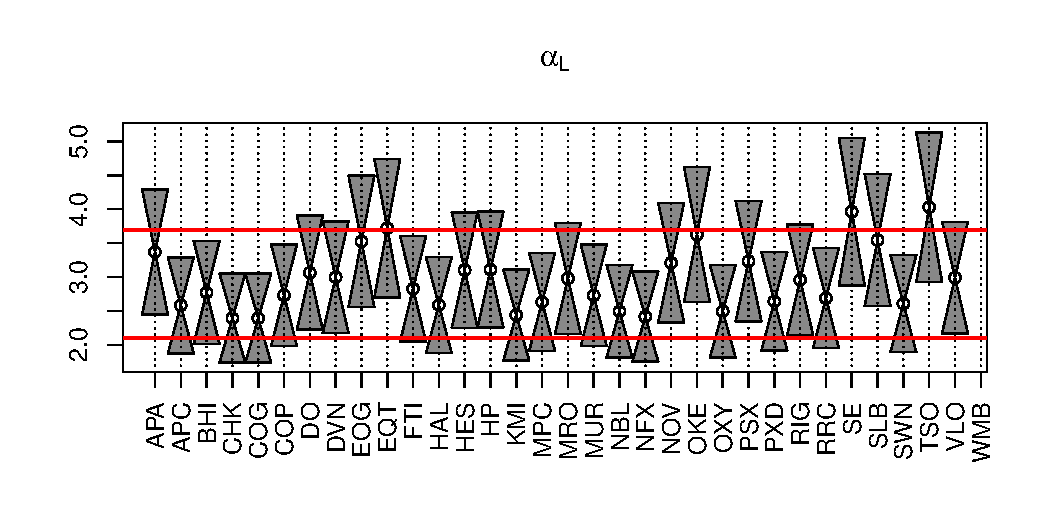
\includegraphics[width=\textwidth, trim={0, 0.8cm, 0, 2cm}, clip]
    {Energy_lower.pdf}
  \end{minipage}
  \begin{minipage}{1.0\linewidth}
    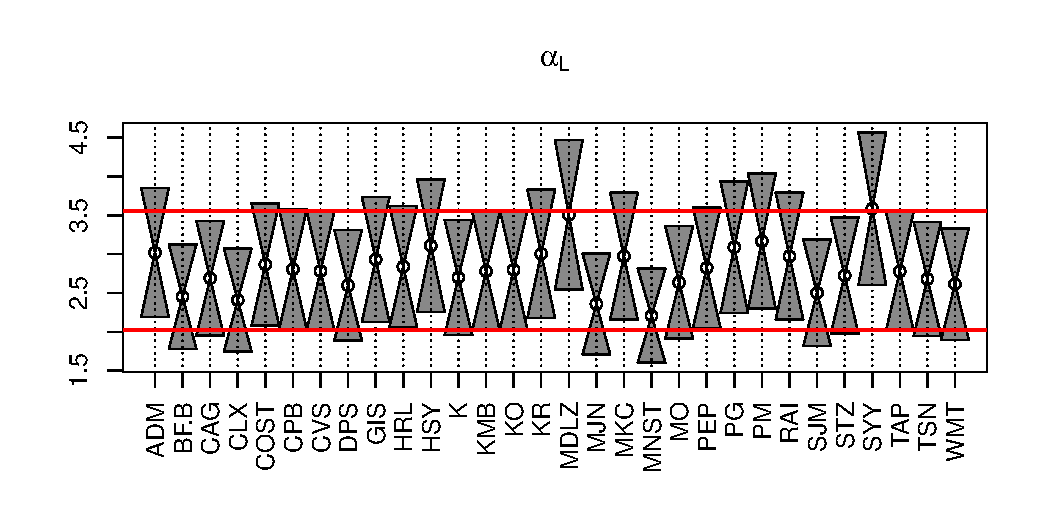
\includegraphics[width=\textwidth, trim={0, 0.8cm, 0, 2cm}, clip]
    {Consumer_Staples_lower.pdf}
  \end{minipage}
  \begin{minipage}{1.0\linewidth}
    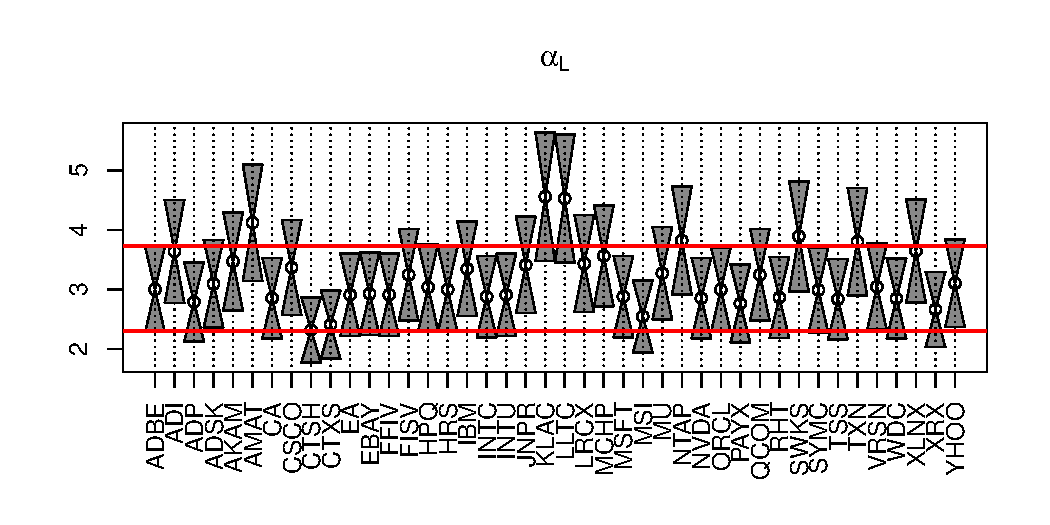
\includegraphics[width=\textwidth, trim={0, 0.8cm, 0, 2cm}, clip]
    {Information_Technology_lower.pdf}
  \end{minipage}
  \caption{\small Hill estimates $\hat \alpha_{50}$ of the lower tail-indices $\alpha$ of
    daily return series in sectors of the S\&P 500
    index. The data span
    from 1 January 2010 to 31 December 2014 and comprise $n=1304$ observations.
The graphs from top to bottom correspond to the ``Energy'',
    ``Consumer Staples'' and ``Information Technology'' sectors.
    Each circle corresponds to a Hill estimate $\hat\alpha_{50}$; the gray
    triangles above and below it mark the 97.5\% and 2.5\% quantiles
    of its approximate normal distribution; see \eqref{eq:2} and the discussion following it for an 
interpretation.
    The lower and upper red lines mark the medians of the 2.5\% 
    and 97.5\% quantiles, respectively, evaluated from all stocks in the sector.
    The data are taken from {\it Yahoo Finance}; the labels on
    the horizontal axes are Yahoo symbols of the stocks. 
  }\label{fig:1}
\end{figure}

In Figure~\ref{fig:1} we see significant overlap of the confidence intervals of the Hill
estimates of the losses in the ``Energy'' and ``Consumer Staples''
sectors of the S\&P 500 index, as well as those of a 
large portion of losses in the ``Information Technology'' sector.
This fact indicates that the returns in each sector may 
have comparable tail-indices.
\par
Hoga's \cite{hoga:2016} test about the change of extreme quantiles
in a sample
may provide some further insight about how similar these tail-indices are.
Different tail-indices are likely to result in different
extreme quantiles. Nevertheless, changes in the extreme quantiles may also
result from changing scale parameters in the tail. Therefore  we first investigate the scale
parameters of daily stock returns in the same sectors of S\&P 500 before we apply the test.


\subsection{Hill estimates of lower-tail scale parameters}\label{sec:HillScaleEstimates}
We assume the pure Pareto model \eqref{eq:3} with scale parameter $K>0$.
Hill \cite{hill1975simple} proposed  the maximum-likelihood estimator of $K$
derived from the joint \ds\ of $k$ upper order statistics in the sample; cf.
Embrechts et al. \cite{embrechts:klueppelberg:mikosch:1997}, p.~334.
It is given by
\beao
\hat K_k = \left({k \over n}\right)^{1/\hat\alpha_k} X_{(n-k)}\,.
\eeao
Using the asymptotic normality property of upper order statistics
(cf. de Haan and Ferreira~\cite{haan:ferreira:2006}, Theorem 2.2.1), one can show
\beao
  \sqrt{k}\, (\hat K_k - K) &\std& N\big(
    0, (K /\alpha)^2\big)\quad\mbox{and}\quad
  \sqrt {k} \,(\hat K_k^\alpha - K^\alpha) \overset{d}{\to} N\big(
    0, K^{2\alpha}  \big)\,,
\end{eqnarray*}
where the tail-index $\alpha$ is regarded as known. From the above
asymptotic normality property, confidence bands of $\hat K_k$
and $\hat K_k^{\hat\alpha}$ can be constructed.   
Estimates $\hat K_k$ in the ``Energy'', ``Consumer Staples'' and
``Information Technology'' sectors of the S\&P 500 index are computed
using this method. The results are shown in
Figure~\ref{fig:sectors_parameters}.
\begin{figure}[htb!]
  \centering
  \begin{minipage}{0.33\linewidth}
    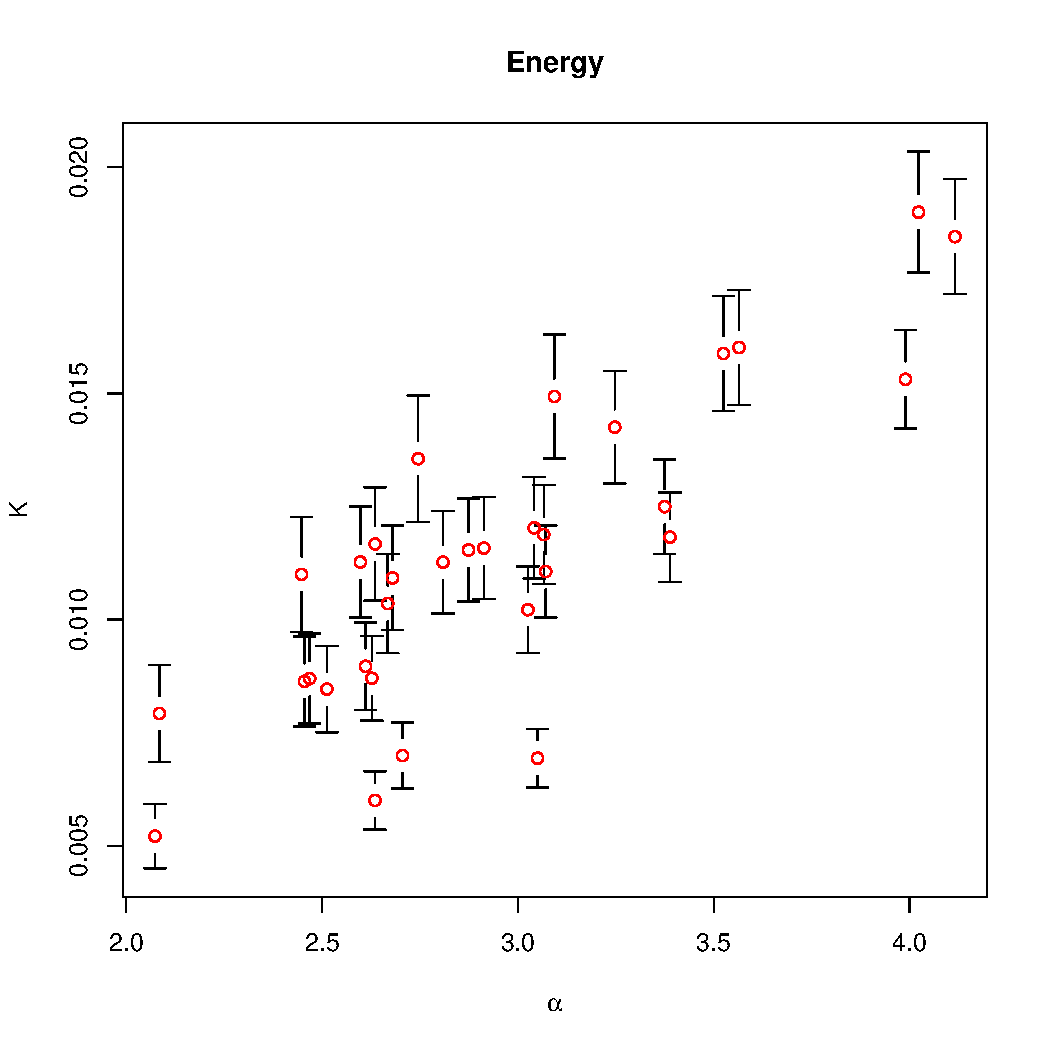
\includegraphics[width=\textwidth]
    {Energy_K.pdf}
  \end{minipage}\hfill
  \begin{minipage}{0.33\linewidth}
    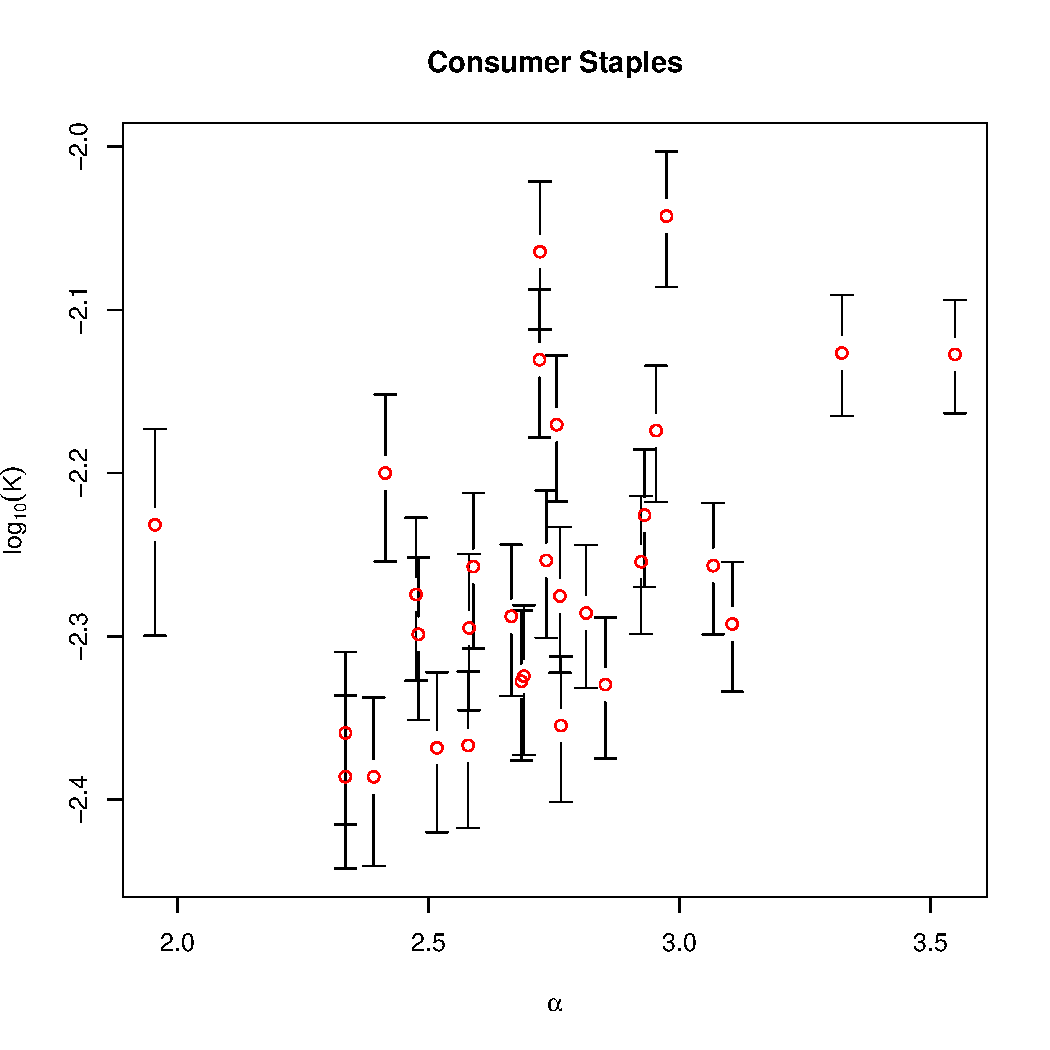
\includegraphics[width=\textwidth]
    {CS_K.pdf}
  \end{minipage}\hfill
  \begin{minipage}{0.33\linewidth}
    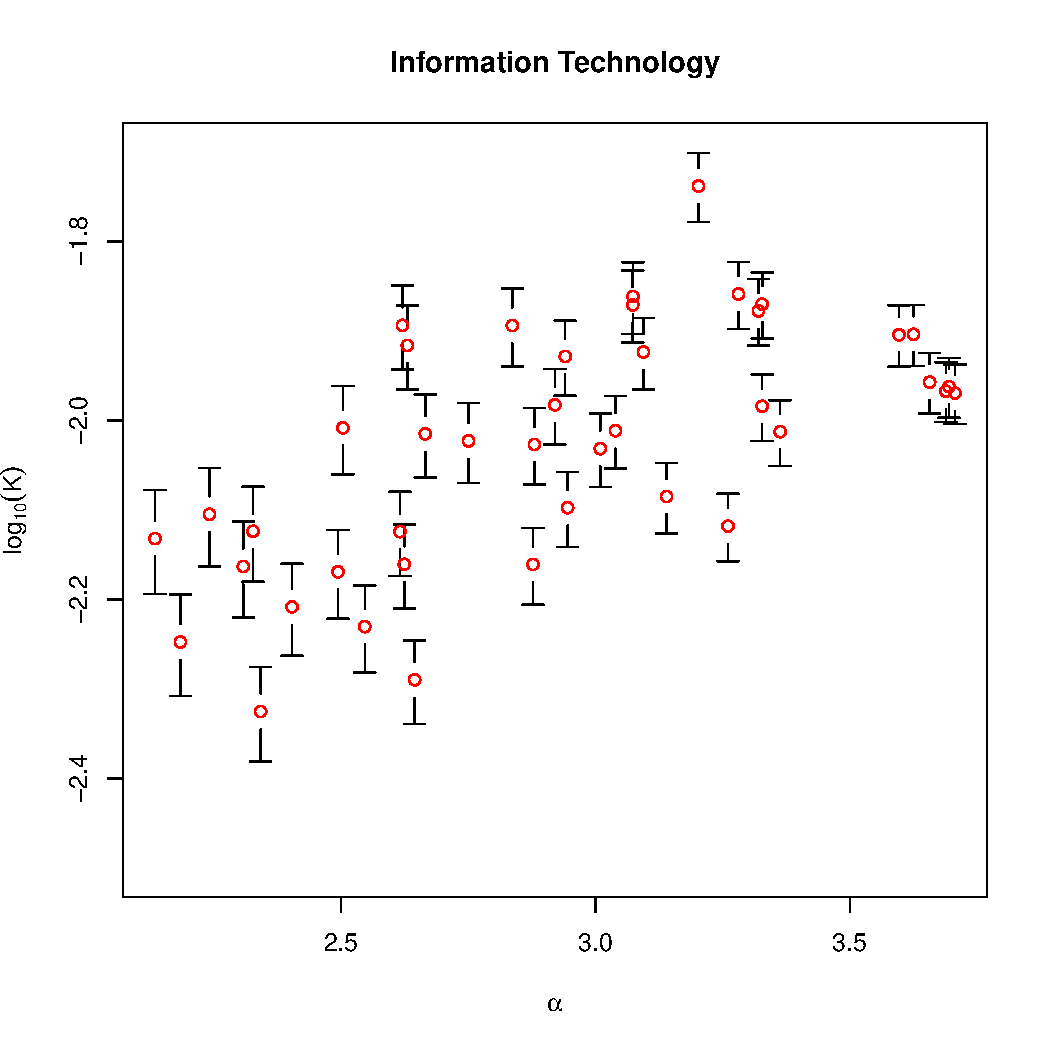
\includegraphics[width=\textwidth]
    {IT_K.pdf}
  \end{minipage}
  \begin{minipage}{0.33\linewidth}
    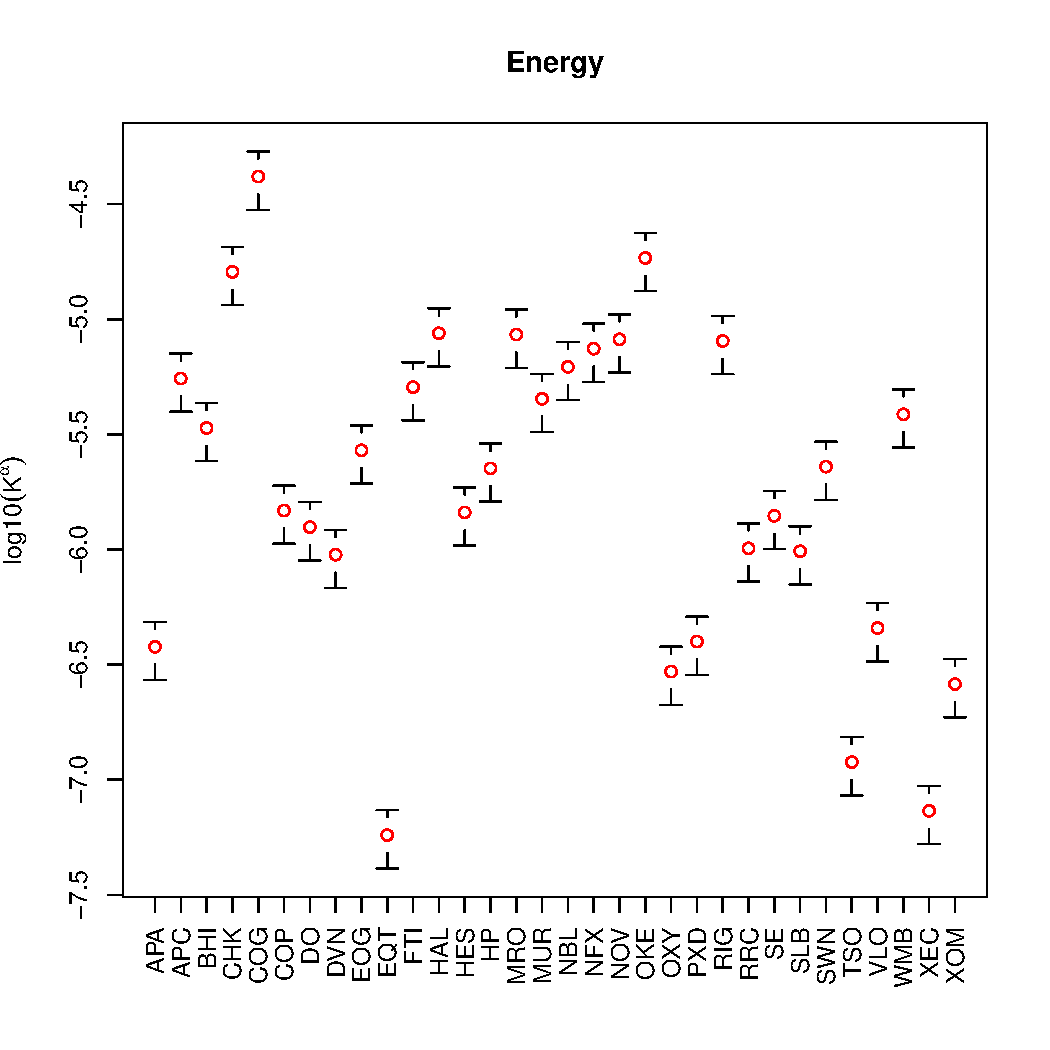
\includegraphics[width=\textwidth]
    {Energy_scale.pdf}
  \end{minipage}\hfill
  \begin{minipage}{0.33\linewidth}
    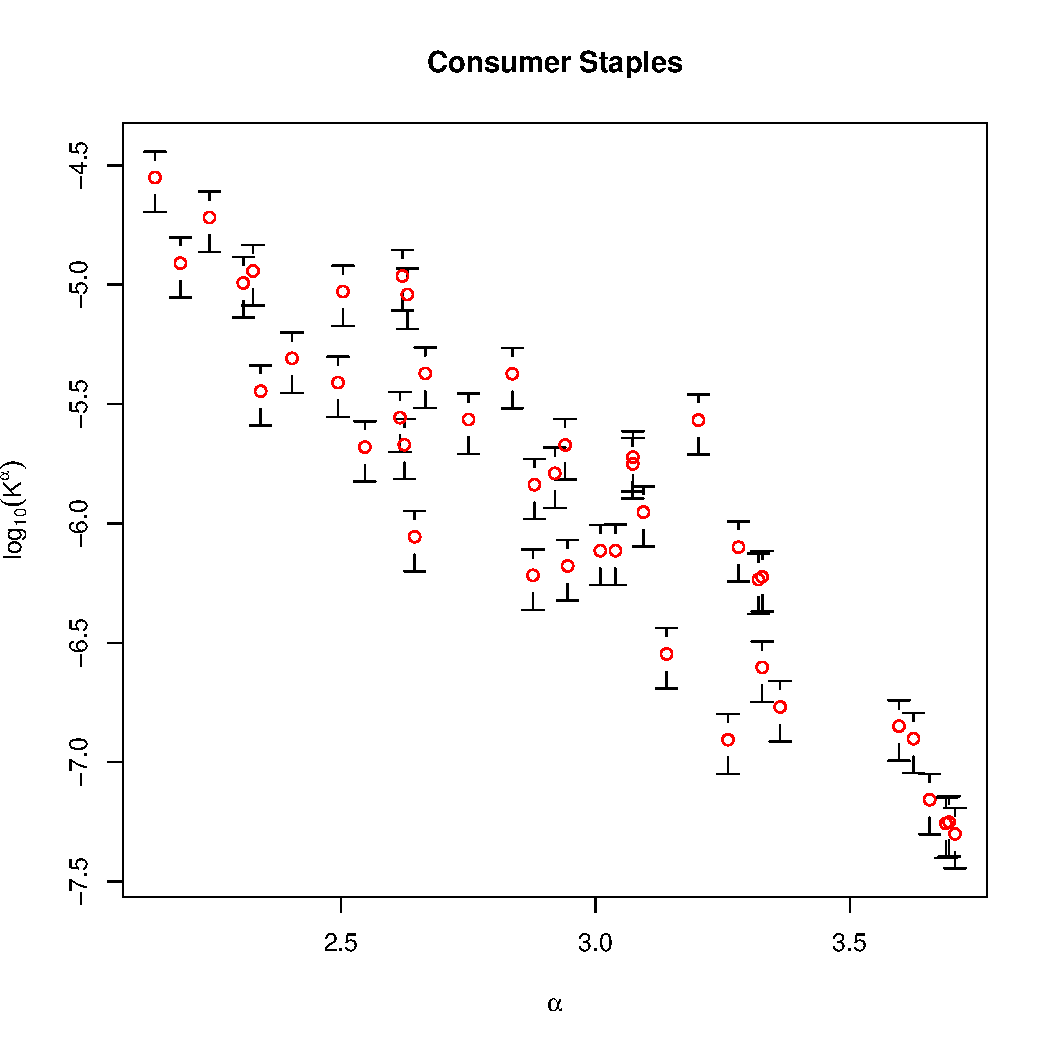
\includegraphics[width=\textwidth]
    {CS_scale.pdf}
  \end{minipage}\hfill
  \begin{minipage}{0.33\linewidth}
    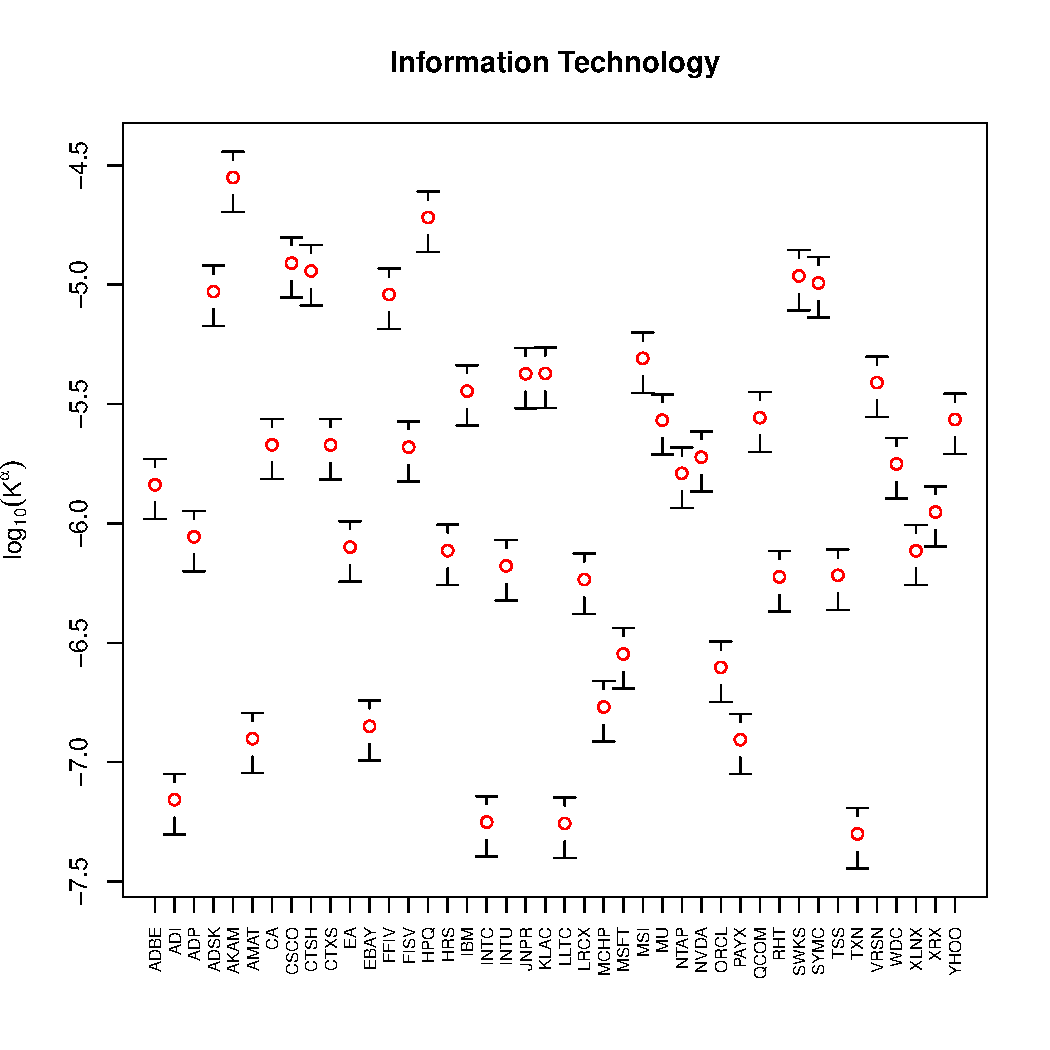
\includegraphics[width=\textwidth]
    {IT_scale.pdf}
  \end{minipage}
  \caption{\small Estimates of $\hat K_k$ (top) and $\hat K_k^{\hat
      \alpha}$ (bottom) on $\log_{10}$-scale of stocks in sectors
    of the S\&P 500 index. The estimates are ordered according to the 
    corresponding estimated $\alpha$-values.
    The points are the estimated values, the bars 
    the \asy\ 95\%-confidence intervals; the confidence bands of the
    corresponding Hill estimates $\hat \alpha_k$ of these sectors are
    shown in Figure~\ref{fig:1}. 
  }
  \label{fig:sectors_parameters}
\end{figure}
One can see that $K$ generally takes a rather small value. For the
more volatile sectors of ``Energy'' and ``Information Technology'',
the average value of $K$ is around 0.01, while for the more stable
sector of ``Consumer Staples'', the average value is around 0.005. Due
to the smallness of $K$, mild variations of $\alpha$ would lead to
huge variations of $K^\alpha$, as shown in the 2nd row of
Figure~\ref{fig:sectors_parameters}.
\par
Secondly, it appears that there is positive dependence between the
values of $\alpha$ and $K$.
As argued in Section~\ref{sec:pareto_tail}, this is consistent with
the assumption that the return series have Pareto tails on both sides
with the tail parameters on each side independent of those on the
other.

\par
Thirdly, Figure~\ref{fig:sectors_parameters} shows that, on
average, the values of $K$
in the ``Energy'' and ``Information Technology'' sectors are  larger
than those in the ``Consumer Staples'' sector.  For a given loss \pro y, 
a larger value of $K$ implies that large losses are more
probable. Thus one can conclude that these two sectors are
considerably riskier than the ``Consumer Staples'' sector. This is of
course a confirmation of one's economic instinct.

Yet another indication from Figure \ref{fig:sectors_parameters} is
that, while the ``Energy'' and the ``Information Technology'' sectors
are similar in riskiness, the dependence  between $\alpha$ and $K$ is
stronger in ``Energy''. As discussed in Section~\ref{sec:3} below, when moving along
a curve of equal preference in the direction of increasing $\alpha$, the parameter $K$ also
increases. So the strong positive dependence seen in the ``Energy''
sector suggests that these stocks might have very similar investor
preferences. This in turn may be attributed to stronger business
relations between the energy enterprises. While two IT companies
may provide a variety of products and services and do not depend on each
other, two energy companies are more likely to depend on each other
via relations of supplier and customer or otherwise to compete with each
other if they are on the same link of the chain of energy production
and distribution.

\subsection{A test for equal tail-indices based on Hill estimation}
Suppose we have two independent strictly stationary positive series $X_1, \dots, X_n $ and
$Y_1, \dots, Y_n$ with corresponding distribution functions $F_X$ and
$F_Y$ that have power-law tails  with indices $\alpha_X$ and
$\alpha_Y$, respectively. From \eqref{eq:2} one can deduce
\begin{equation}
  \label{eq:x3}
  \sqrt k
  \begin{pmatrix}
    {\hat \alpha_X - \alpha_X} \\
    {\hat \alpha_Y - \alpha_Y} \\
  \end{pmatrix} \overset{d}{\to}
  \begin{pmatrix}
    Z_X \\
    Z_Y
  \end{pmatrix}
  \sim
  N\left(
    0, \text{diag}(\alpha_X^2, \alpha_Y^2)
  \right)
\end{equation}
where $\hat \alpha_X$ and $\hat \alpha_Y$ are Hill estimators of
$\alpha_X$ and $\alpha_Y$; we suppress their dependence on $k$. Then it follows from the continuous mapping
theorem
\begin{equation}
  \label{eq:x1}
  \sqrt k [(\hat \alpha_X -\alpha_X) - (\hat \alpha_Y - \alpha_Y)]
  \overset{d}{\to}
  Z_X - Z_Y \sim N(0, \alpha_X^2 + \alpha_Y^2)\,.
\end{equation}
This relation allows one to construct an \asy\ test under 
the null hypothesis $\alpha_X = \alpha_Y$ and with test statistic $\hat \alpha_X - \hat \alpha_Y$.
We apply this test to the equities in the ``Energy'',
``Consumer Staples'' and ``Information Technology''
sectors of the S\&P 500 index. The results are shown in the top row of
Figure~\ref{fig:PairTest}.
\begin{figure}[htb!]
  \begin{minipage}{0.33\linewidth}
    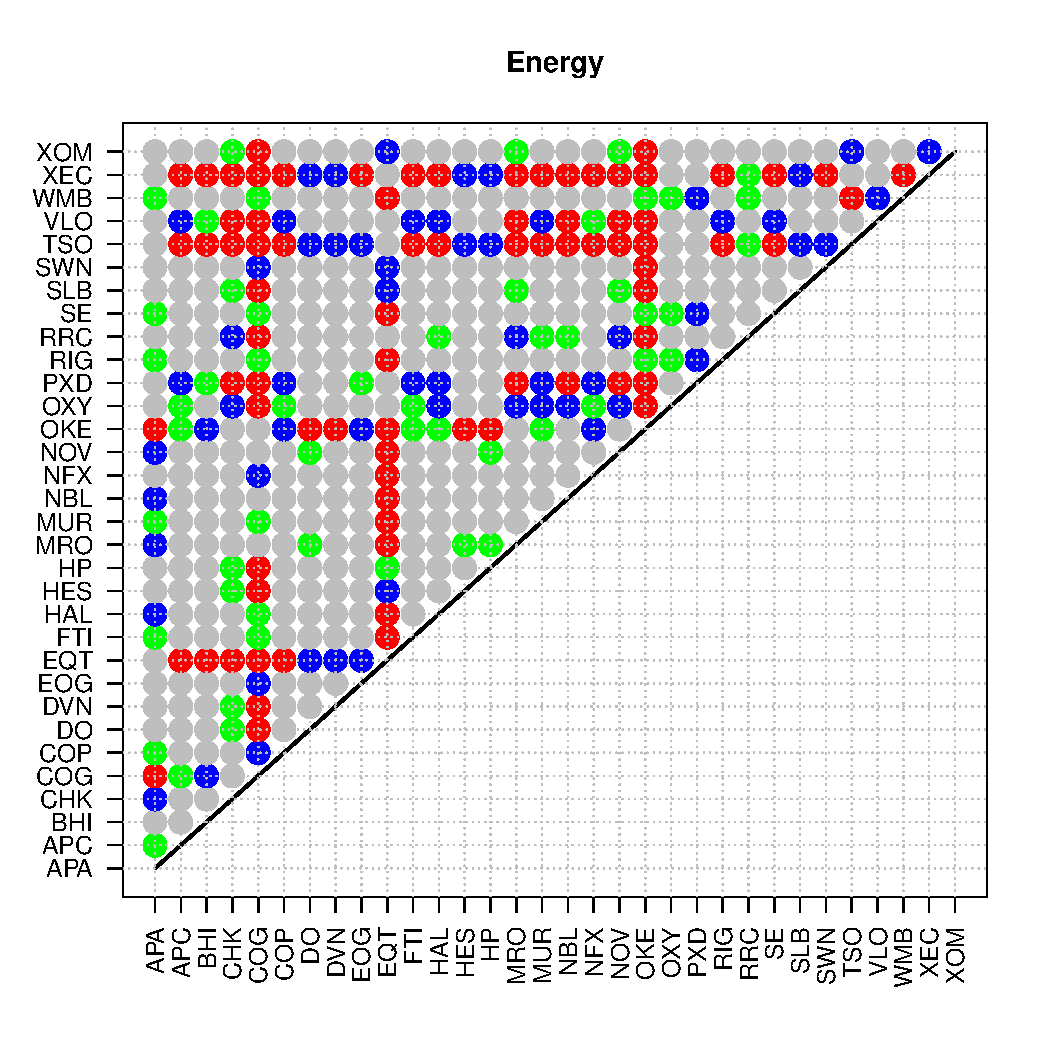
\includegraphics[
      width=\textwidth,
      trim={0.3cm, 0.8cm, 1cm, 0.6cm}, clip
    ]{HillTest_Energy.pdf}
  \end{minipage}\hfill
  \begin{minipage}{0.33\linewidth}
    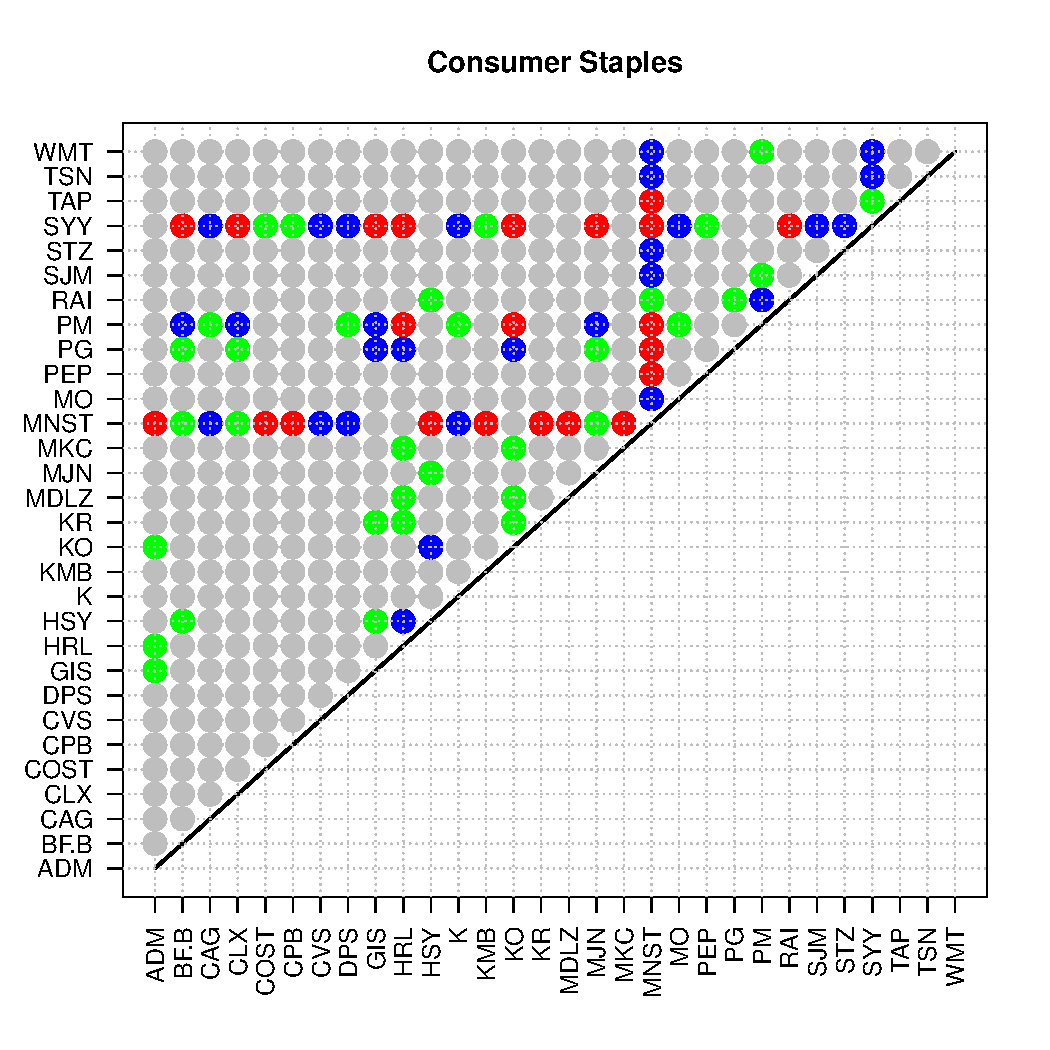
\includegraphics[
      width=\textwidth,
      trim={0.3cm, 0.8cm, 1cm, 0.6cm}, clip
    ]{HillTest_CS.pdf}
  \end{minipage}\hfill
  \begin{minipage}{0.33\linewidth}
    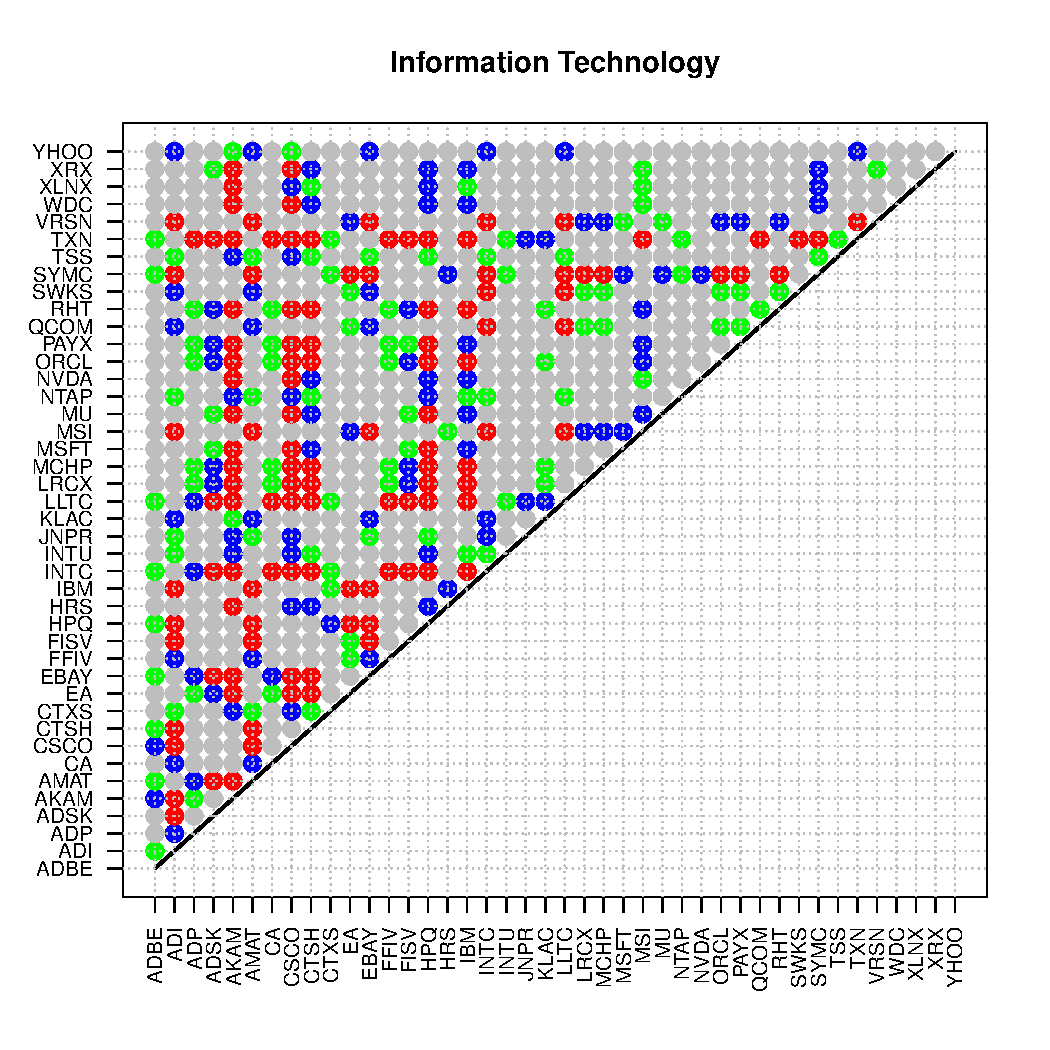
\includegraphics[
      width=\textwidth,
      trim={0.3cm, 0.8cm, 1cm, 0.6cm}, clip
    ]{HillTest_IT.pdf}
  \end{minipage}
  \begin{minipage}{0.33\linewidth}
    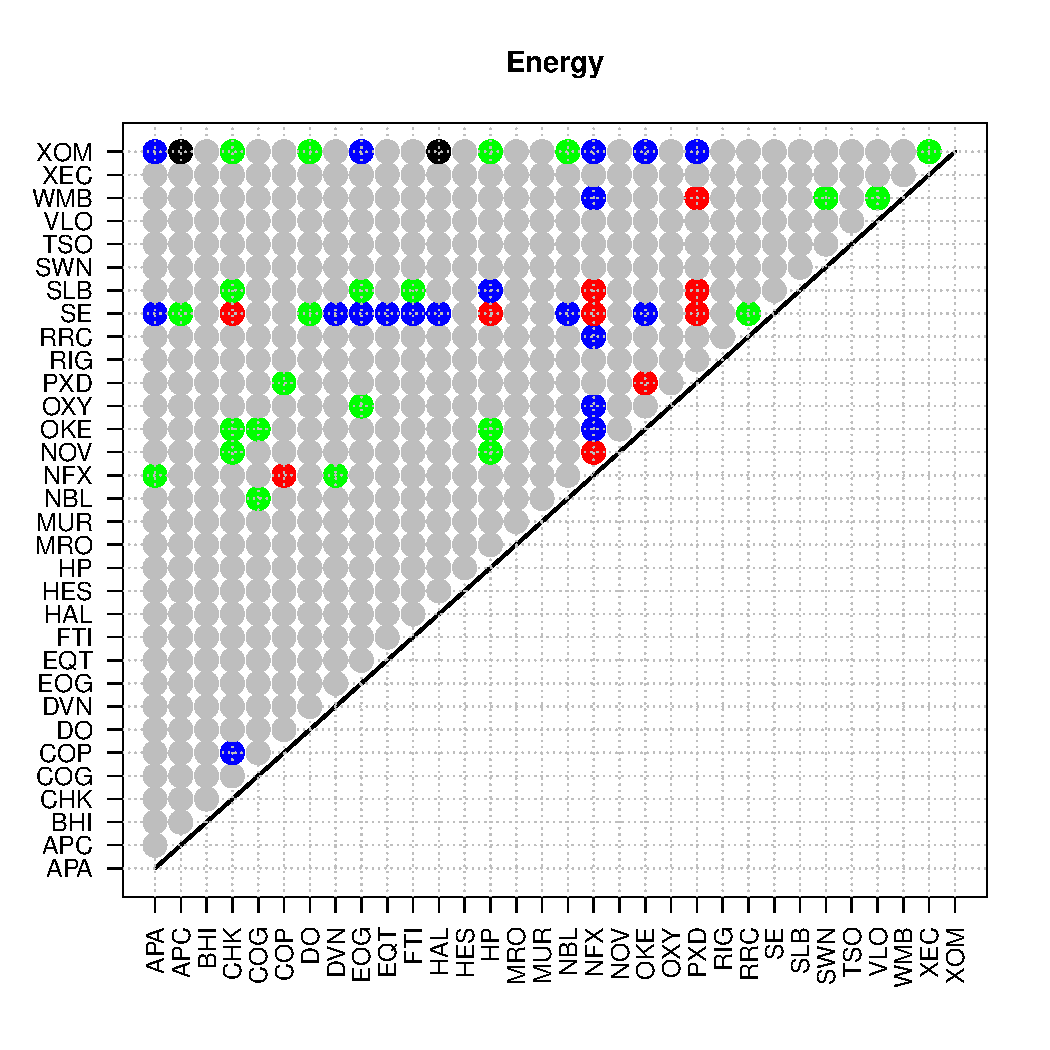
\includegraphics[
      width=\textwidth,
      trim={0.3cm, 0.8cm, 1cm, 0.6cm}, clip
    ]{Hoga_Energy_pair.pdf}
  \end{minipage}\hfill
  \begin{minipage}{0.33\linewidth}
    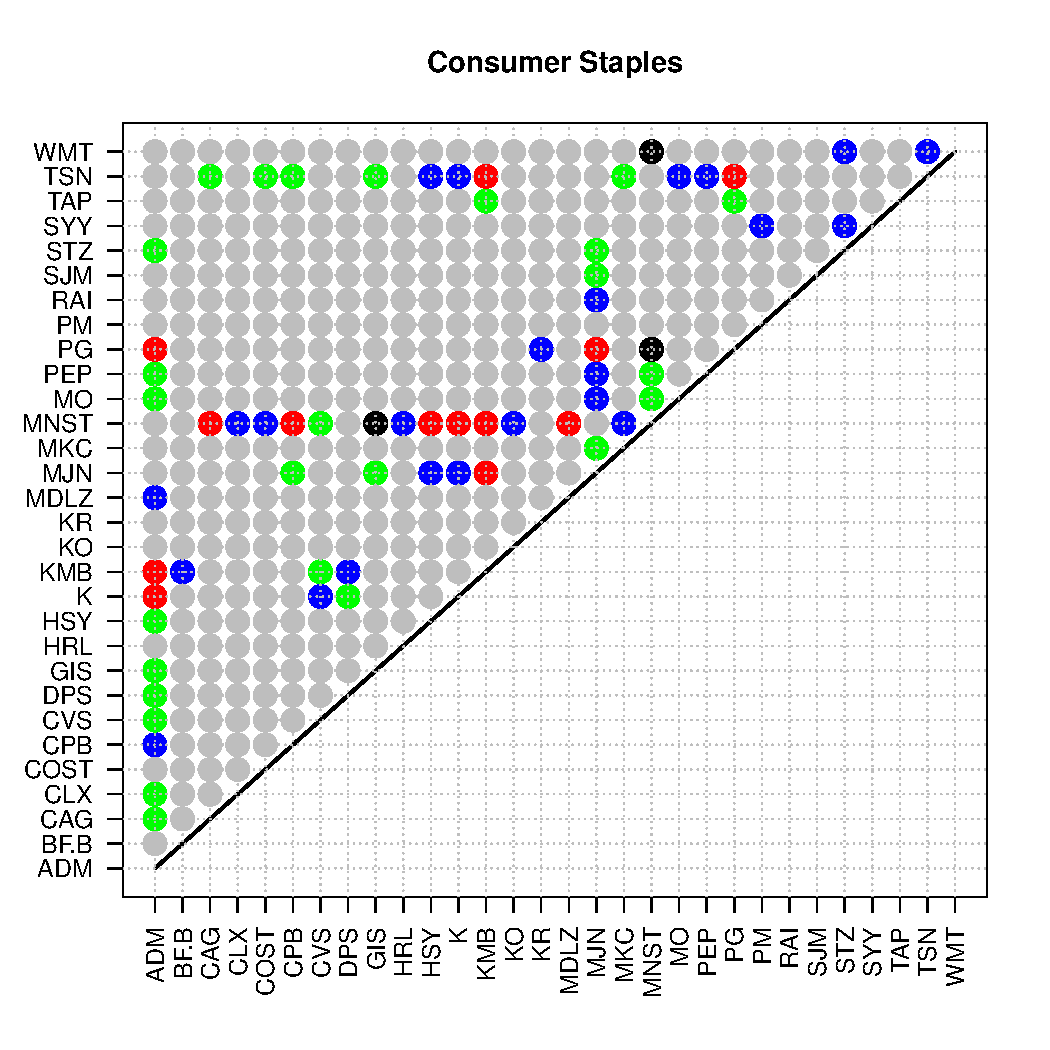
\includegraphics[
      width=\textwidth,
      trim={0.3cm, 0.8cm, 1cm, 0.6cm}, clip
    ]{Hoga_CS_pair.pdf}
  \end{minipage}\hfill
  \begin{minipage}{0.33\linewidth}
    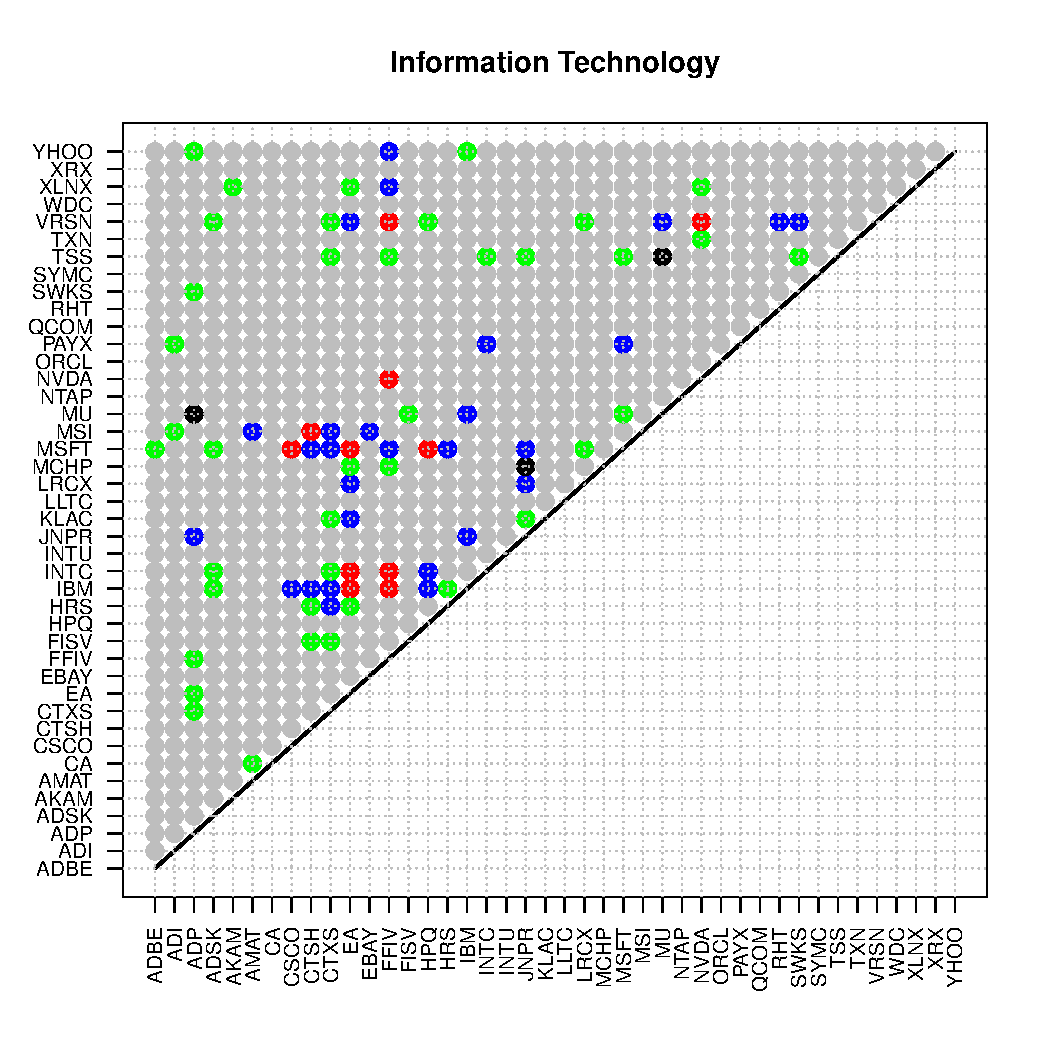
\includegraphics[
      width=\textwidth,
      trim={0.3cm, 0.8cm, 1cm, 0.6cm}, clip
    ]{Hoga_IT_pair.pdf}
  \end{minipage}
  \caption{{\em Top row}: Test for pairwise equality of tail-indices
    of losses in the  ``Energy'', ``Consumer Staples'' and
    ``Information Technology'' 
    sectors of S\&P 500. The test statistic in $\hat\alpha_X-\hat \alpha_Y$ is based
    on Hill estimates 
    of $\alpha_X$ and $\alpha_Y$. 
    The green, blue and red points correspond to pairs of stock in a sector
    when the test statistic is outside the intervals $[q_{0.075},q_{0.925}]$,
    $[q_{0.05},q_{0.95}]$,  $[q_{0.025},q_{0.975}]$, respectively, where
    $q_p$ is the $p$-quantile of the limiting 
    $N(0,\alpha_X^2+\alpha_Y^2)$-\ds\ of the test statistic in
    \eqref{eq:x1}. Grey points stand for pairs for which the test
    statistic is inside $[q_{0.075},q_{0.925}]$. 
    {\em Bottom row:} Test for changing tail-index or scale parameter
    of losses
    using Hoga's test based on concatenated series of pairs of
    stocks. The green, blue and red points
    correspond to pairs of stock in a sector 
    when the test statistic $T_n$ exceeds the $85\%$-, $90\%$-,
    $95\%$-quantile of the limit \ds .
  Grey points stand for pairs for which the test statistic is below
  the \asy\ $85\%$-quantile. Black points represent 
    pairs for which the computation of $T_n$ fails for given precision  
    requirements and time limits.
    The same number (50) of upper order statistics is used for both tests.}
  \label{fig:PairTest} 
\end{figure}
They indicate that tail-indices of equities in the
``Energy'' or ``Information Technology'' sectors are more variable 
than in the ``Consumer Staples'' sector, as the null
hypothesis is rejected more often for members of these two former sectors.
Moreover, these figures suggest that the test based on the Hill estimator
is quite powerful in distinguishing between tail-indices. In contrast to the test presented in Section~\ref{sec:Hoga}
the present test results in  more rejections for the ``Energy'' and the
``Information Technology'' sectors.
\par
As a caution, one should bear in mind that 
\eqref{eq:x3} is valid on condition that the $X$- and $Y$-
series are independent of each other (or weakly dependent on each other), which is generally untrue for
two return series in the same market.

\subsection{A test for a change in the extreme tail}\label{sec:Hoga}
Here we apply a test from
a recent paper by Hoga \cite{hoga:2016}. This test has been developed
for a different kind of problem. Given a strictly stationary
\ts\ $X_1,\ldots,X_n$ with a marginal \ds\ $F$ with right power-law
tail, the goal is to test whether there is a structural break of the
{\em extreme quantiles} $F^{-1}(1-p)$ for values $p$ very close to
zero. If the tail-index {\em or} the scale parameter in a \ds\ of type
\eqref{eq:3} change inside a sample, then it is likely that the
extreme quantiles change as well. We will test for a change of tail-index or scale parameter in this indirect way.
\par
The null hypothesis of the test in \cite{hoga:2016} is that there is no change of the extreme quantiles $F^{-1}(1-p)$ 
for $p=p_n\to 0$ in any subsample with indices
$t\in (n\,t_0,n(1-t_0))$ where $t_0$ is a fixed number in $(0,0.5)$. Writing $\hat x_p(a,b)$ for an estimator of the extreme $(1-p)$-quantile 
based on the subsample with indices $t\in (na,nb)$, the test statistic is given by
\beam\label{eq:4}
T_n = \sup_{s \in [t_0, 1 - t_0]}
  \dfrac{  \big[s (1 - s) \log \big(\hat x_p(0, s)/\hat x_p(s, 1)\big)
    \big]^2}{
    \int_{t_0}^s\big[r \log \big( \hat x_p(0, r)/\hat x_p(0, s)
      \big)
    \big]^2 dr
    +
    \int_{s}^{1 - t_0}
    \big[
      (1 - r) \log \big(
      \hat x_p(r, 1)/
      \hat x_p(s, 1)
      \big)
    \big]^2 dr}\nonumber\\
\eeam
Under the null hypothesis, $(T_n)$ converges to a complicated \fct al
of Brownian motion\ on $[0,1]$; the \asy\ quantiles need to be
evaluated by simulation.
\par
When applied to our problem we would like to test 
whether there is a change of the tail-index {\em or} scale parameter in \eqref{eq:3} in each of the S\&P 500 
series in the distinct sectors. We also  want to get some indication about a possible change of tail-index or
scale parameter from one series to another within a given sector. For this reason, we choose any pair of series
within a sector and concatenate each of the paired series. Then we run the test on the concatenated series.
Of course, despite the fact that we test changes of tail-index or scale parameter 
{\em in a very indirect way} -- there may be many other reasons for the change of extreme quantiles in a sample -- 
we also concatenate two rather distinct series. Even if we assume that the two series come from related models
(such as GARCH), the parameters of these models will in general not be the same. Moreover, the concatenation
of two strictly stationary \ts\ is in general not strictly stationary. Therefore we have to be careful
with interpretations of the results of the tests.
\par 
In Figure~\ref{fig:Hoga_Single} we show the values of the test statistic $T_n$ (horizontal bars)
for $t_0=0.1$ and daily return series of stock in the ``Energy'' and ``Consumer Staples'' sectors of the S\&P
500 index. The ``null hypothesis'' is that the tail-index and scale parameter remain the
same throughout the selected period of time. For most stocks, the hypothesis cannot be rejected even at the 85\% level.
This fact may be an indication that the \ds\ inside a series is rather homogeneous.
Alternatively, it may show that the power of the test is very low. A possible reason for this suspicion is that the \con\ rate
of $(T_n)$ to its limit is very slow, i.e., the \asy\ \ds\ is not representative for the \ds\ of $T_n$ for the chosen $n$; for some
simulation evidence, see below.
\par
To check whether any pair of stocks shares the same tail-index and scale parameter we concatenate
any two series and apply the aforementioned test on the concatenated series. For the ``Energy'' and the
``Consumer Staples'' sector we summarize the results in the bottom row of Figure~\ref{fig:PairTest}.
These graphs show that the ``null
hypothesis'' of an equal tail-index and scale parameter is rejected for more pairs in the
``Energy'' sector than it is for those in the ``Consumer Staples''
sector. This suggests that lower tail-indices of stocks in the
``Energy'' sector are more spread out than those of the ``Consumer
Staples'' sector. Also observe that while 3 stocks, say A, B and C, test in favor of
the relations $\alpha_A = \alpha_B, \alpha_A \neq \alpha_C$, it often
happens that another test on B and C is supportive of $\alpha_B = \alpha_C$. Again,
this is due to the limited power of the test. Based
on such results, one may guess that $\alpha_B$ lies between $\alpha_A$ and
$\alpha_C$. The test is unable to recognize the smaller differences
between $\alpha_A, \alpha_B$ on one hand and between $\alpha_B, \alpha_C$ on the other hand.
\begin{figure}[htb!]
  \begin{minipage}{0.5\linewidth}
    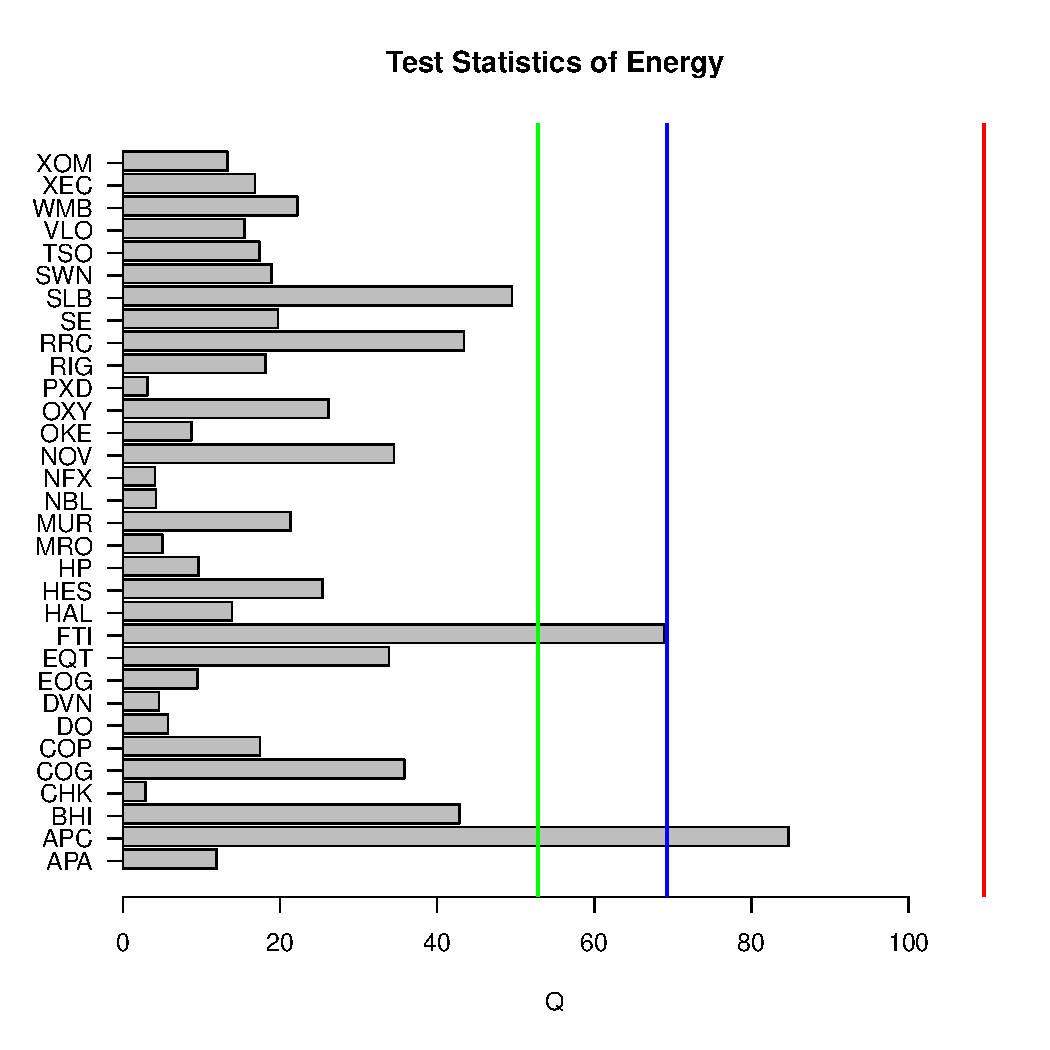
\includegraphics[width=\textwidth]
    {Hoga_Energy_Single.pdf}
  \end{minipage}\hfill
  \begin{minipage}{0.5\linewidth}
    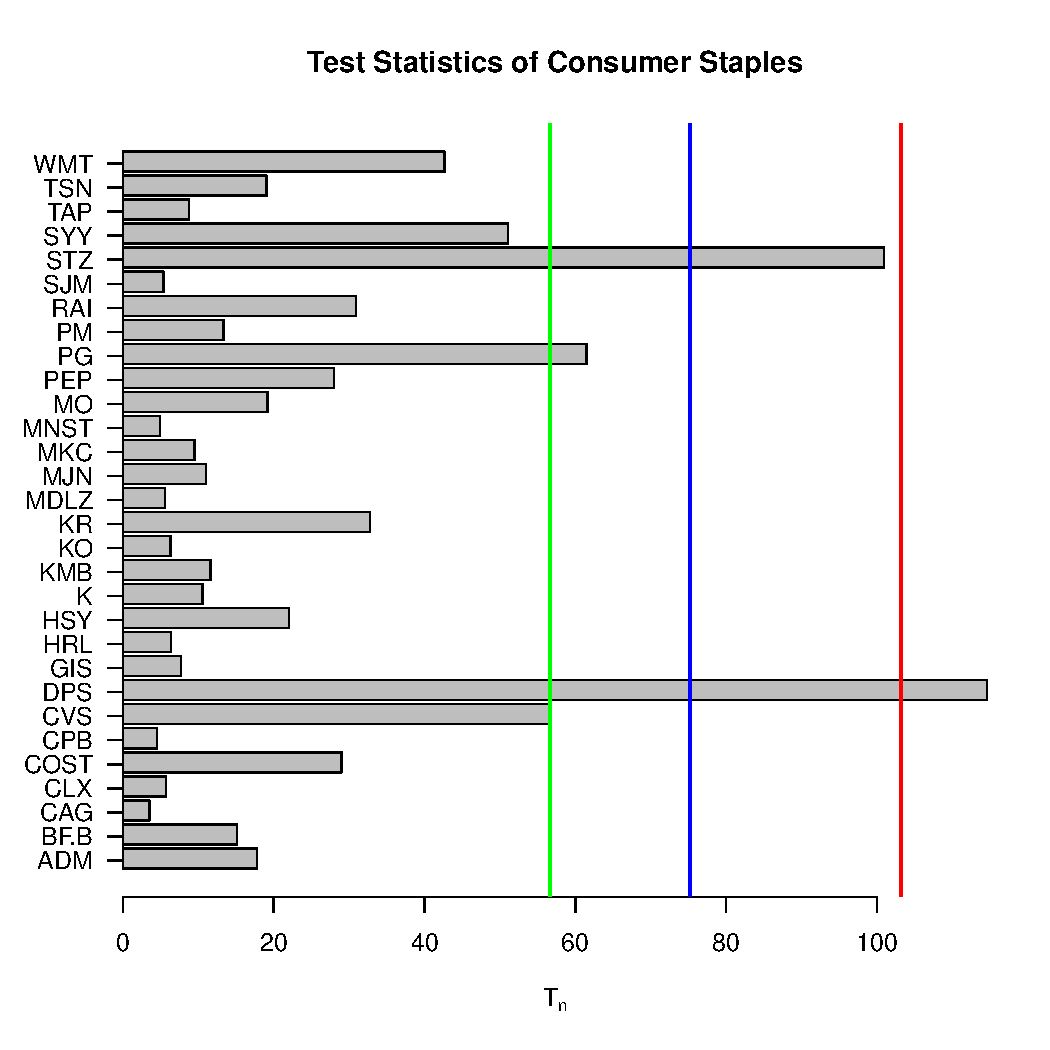
\includegraphics[width=\textwidth]
    {Hoga_CS_Single.pdf}
  \end{minipage}
  \caption{Test statistic $T_n$ from \eqref{eq:4} for the  stocks in the ``Energy'' and
    ``Consumer Staples'' sectors of S\&P 500. The green, blue and red
    lines correspond to the 85\%, 90\% and 95\% quantiles of the limit \ds\ of $T_n$.  They are derived
by simulations from the limit \ds .}
  \label{fig:Hoga_Single}
\end{figure}

To get an idea about the power of the test we run it on a
sample concatenated from two independent iid samples of the same size
$n=1304$ as the S\&P 500 series. Both pieces are $t$-distributed with
distinct degrees of freedom. The results are shown in
Figure~\ref{fig:t_sim_pair}: the power of the test is the smaller the
larger the minimum tail-index in the concatenated pair.
\begin{figure}[htb!]
  \begin{minipage}{0.5\linewidth}
    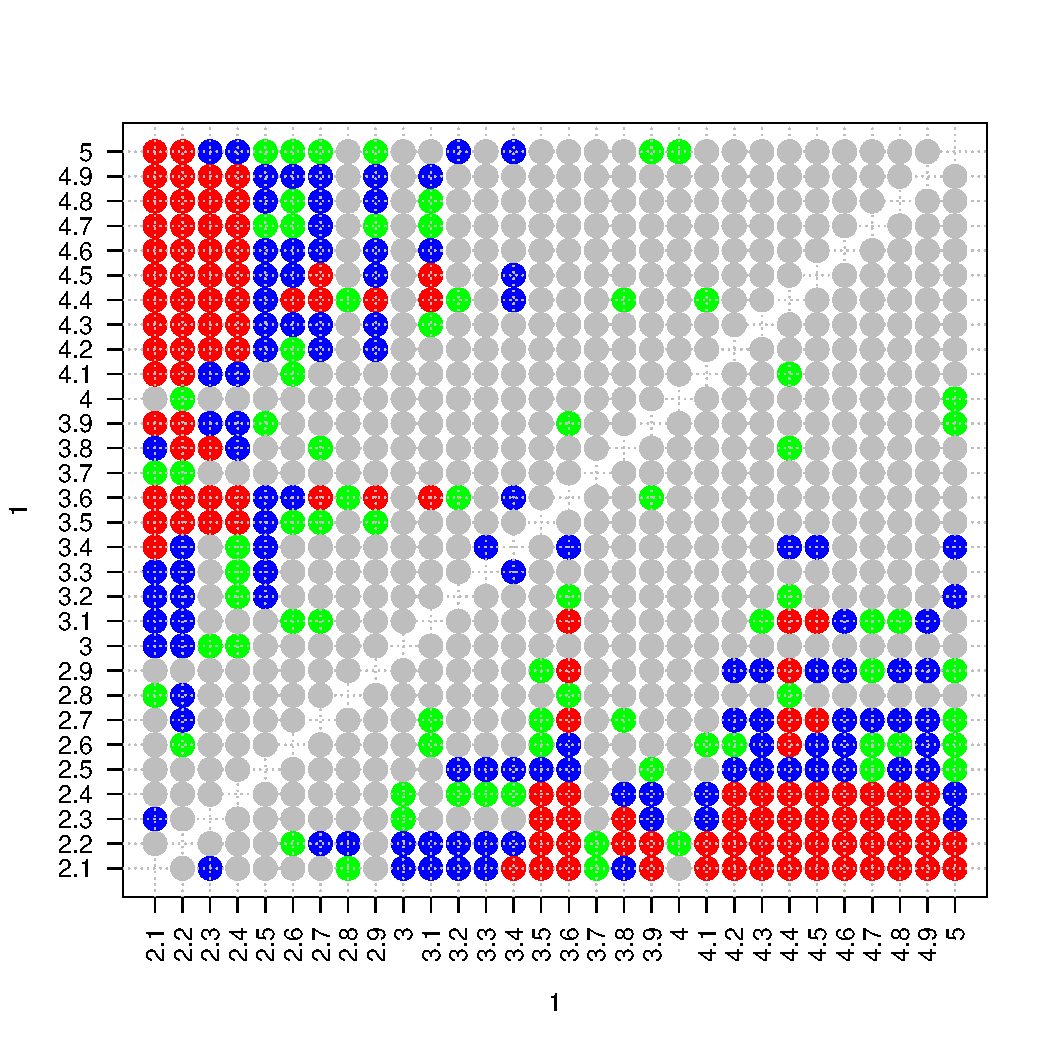
\includegraphics[width=\textwidth]{t_sim_pair.pdf}
  \end{minipage}\hfill
  \begin{minipage}{0.5\linewidth}
    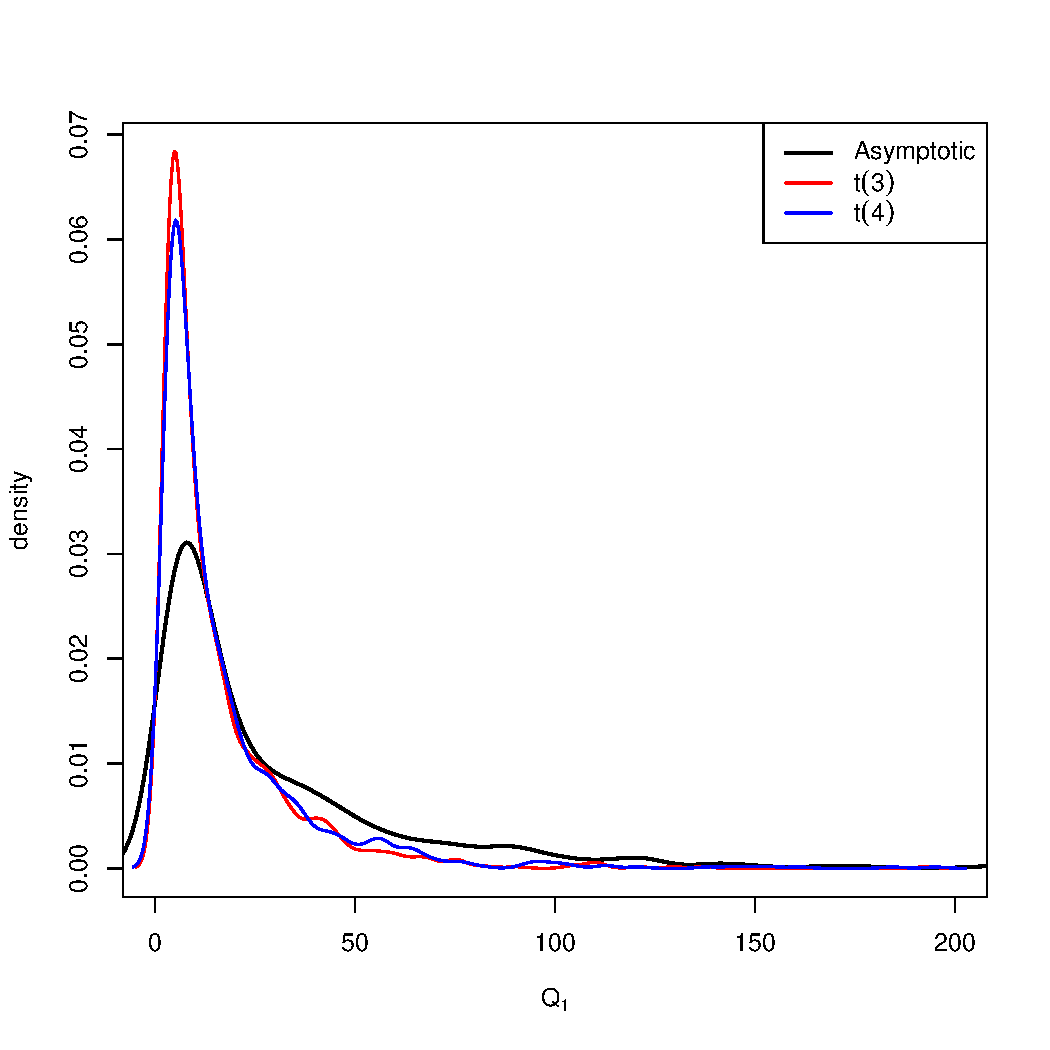
\includegraphics[width=\textwidth]{Hoga_AsymptoticDistribution.pdf}
  \end{minipage}
  \caption{
    {\em Left}: Test  of concatenated $t$-samples with different
    degrees of freedom $\alpha$. Numbers on the axes are the degrees of freedom
    in the subsamples. For an interpretation of the colored bullets,
    see the caption for the bottom row of Figure~\ref{fig:PairTest}. The graph shows the limited power
    of the test. In particular, if both degrees of freedom are
    relatively large it loses the capability of distinguishing between the \ds s.
    {\em Right}: Comparison of the \asy\ distribution of the test statistic
    $T_n$ in \eqref{eq:4} under the null hypothesis and the \ds\ of
    $T_n$ for $n=1304$ iid $t$-distributed $X_t$ with 3 and 4 degrees
    of freedom.
  }
  \label{fig:t_sim_pair}
\end{figure}

A major problem of this test is the \asy\ distribution of the test statistic under the
null hypothesis.  The rate at which the finite-sample distribution tends to its limit is not known.
To find out about this problem we compared the \ds s of $T_{1304}$ 
for $t$-distributed $X_t$ with  $\alpha=3$ and $\alpha=4$ degrees of freedom with
the limit \ds\ of $T_n$.
The estimated density functions are shown on the right of Figure~\ref{fig:t_sim_pair}.
As seen in the graph, the asymptotic distribution assigns
significantly more mass to the tail than the \ds s of $T_n$ do. For
comparison, we list a few quantiles of these \ds s in
Table~\ref{tab:HogaAsymptotic}, showing major differences between the
\asy\ and finite-sample \ds s.
\begin{table}[htb!]
  \centering
  \begin{tabular}{l|c|c|c|r}
    & \multicolumn{4}{c}{Quantiles} \\[2mm]
    \hline
    Distribution of $X_t$& 80\% & 85\% & 90\% & 95\% \\
    \hline
    Asymptotic & 47.48 & 59.61 & 78.90 & 113.12 \\
    t(3)  & 23.30 & 28.27 & 35.04 & 46.75 \\
    t(4)  & 25.76 & 31.13 & 38.81 & 56.32\\[2mm]
  \end{tabular}
  \caption{Quantiles of the test statistic $T_n$ for $n=1304$
    $t$-distributed samples with $\alpha=3$ and $\alpha=4$ 
degrees of freedom
    as well as the corresponding quantiles for the limiting \ds\ of
    $T_n$. In particular, there are huge differences between the three
    \ds s  for the higher quantiles. 
    }
  \label{tab:HogaAsymptotic}
\end{table}

Figure~\ref{fig:PairTest:permuted} points at another shortcoming
of the test: we show $T_n$ for an 
arbitrarily chosen random permutation of the concatenated data from two 
different stocks. In this case the null hypothesis that two series
have the same tail-index is rejected much more often, as a comparison
with the bottom graphs of
Figure~\ref{fig:PairTest} shows. If the data in the concatenated 
series were iid a random permutation would not change the 
\ds\ of $T_n$. Thus the value of the test statistic $T_n$  
strongly depends on the dependence structure of the underlying data
and therefore a test based on $T_n$ may be misleading.

\begin{figure}[htb!]
  \begin{minipage}{0.33\linewidth}
    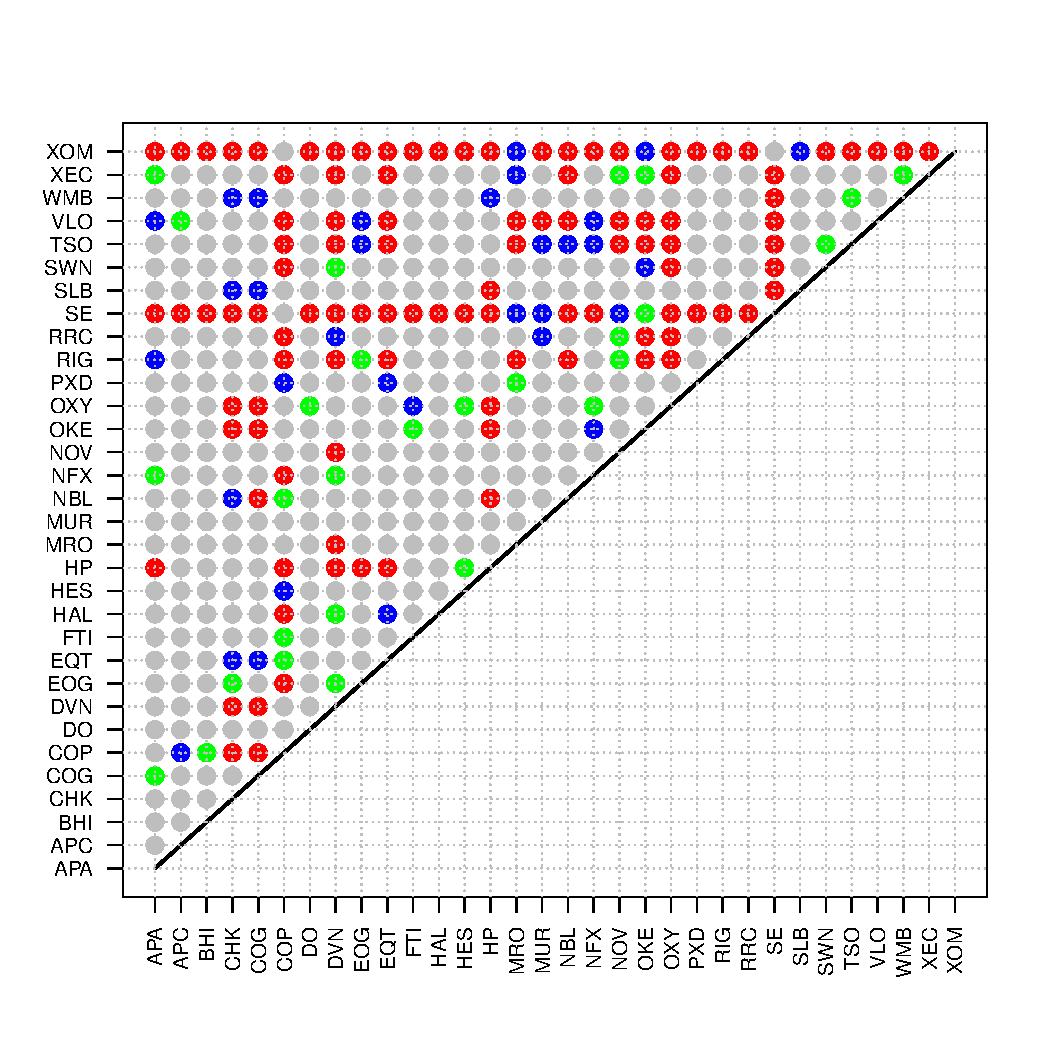
\includegraphics[
      width=\textwidth,
      trim={0.3cm, 0.8cm, 1cm, 0.6cm}, clip
    ]{Hoga_Energy_pair_permuted.pdf}
  \end{minipage}\hfill
  \begin{minipage}{0.33\linewidth}
    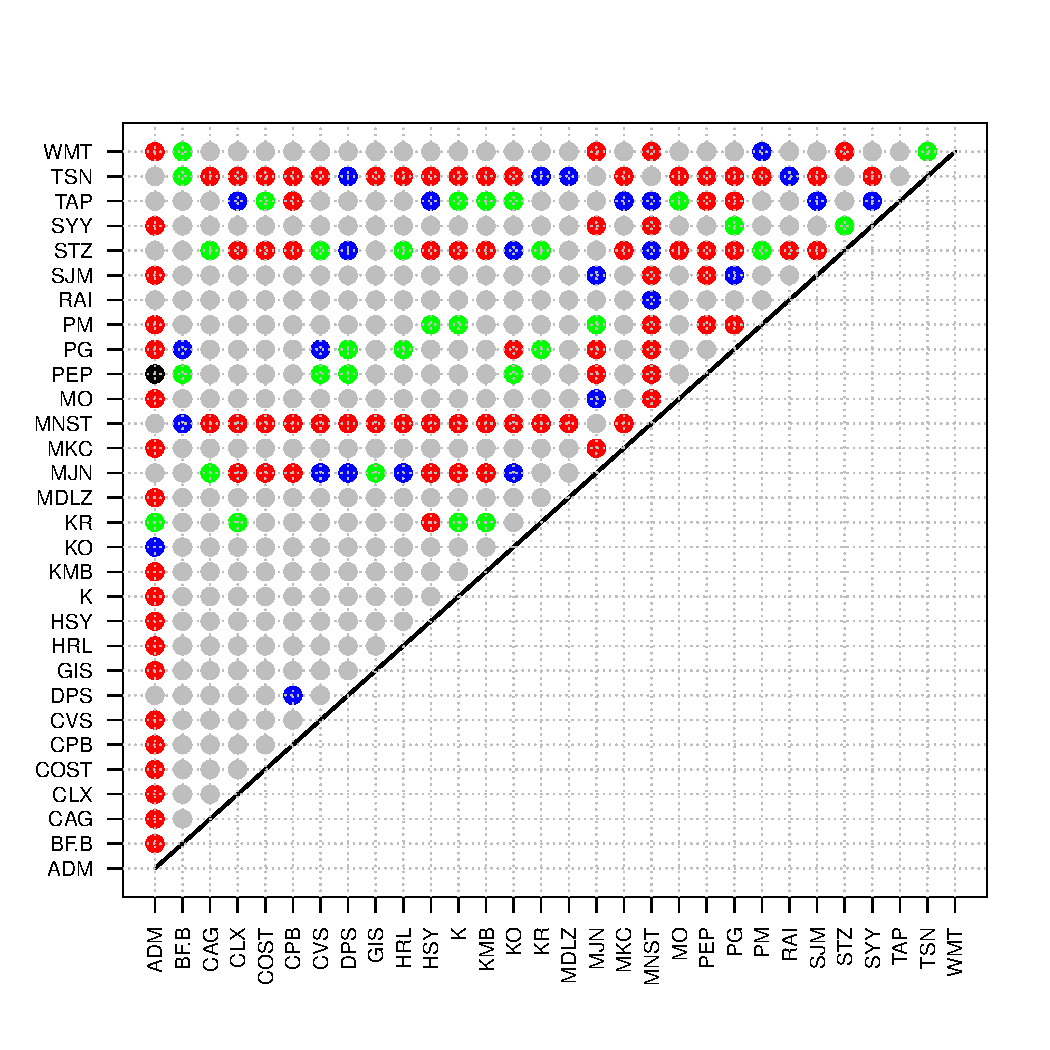
\includegraphics[
      width=\textwidth,
      trim={0.3cm, 0.8cm, 1cm, 0.6cm}, clip
    ]{Hoga_CS_pair_permuted.pdf}
  \end{minipage}\hfill
  \begin{minipage}{0.33\linewidth}
    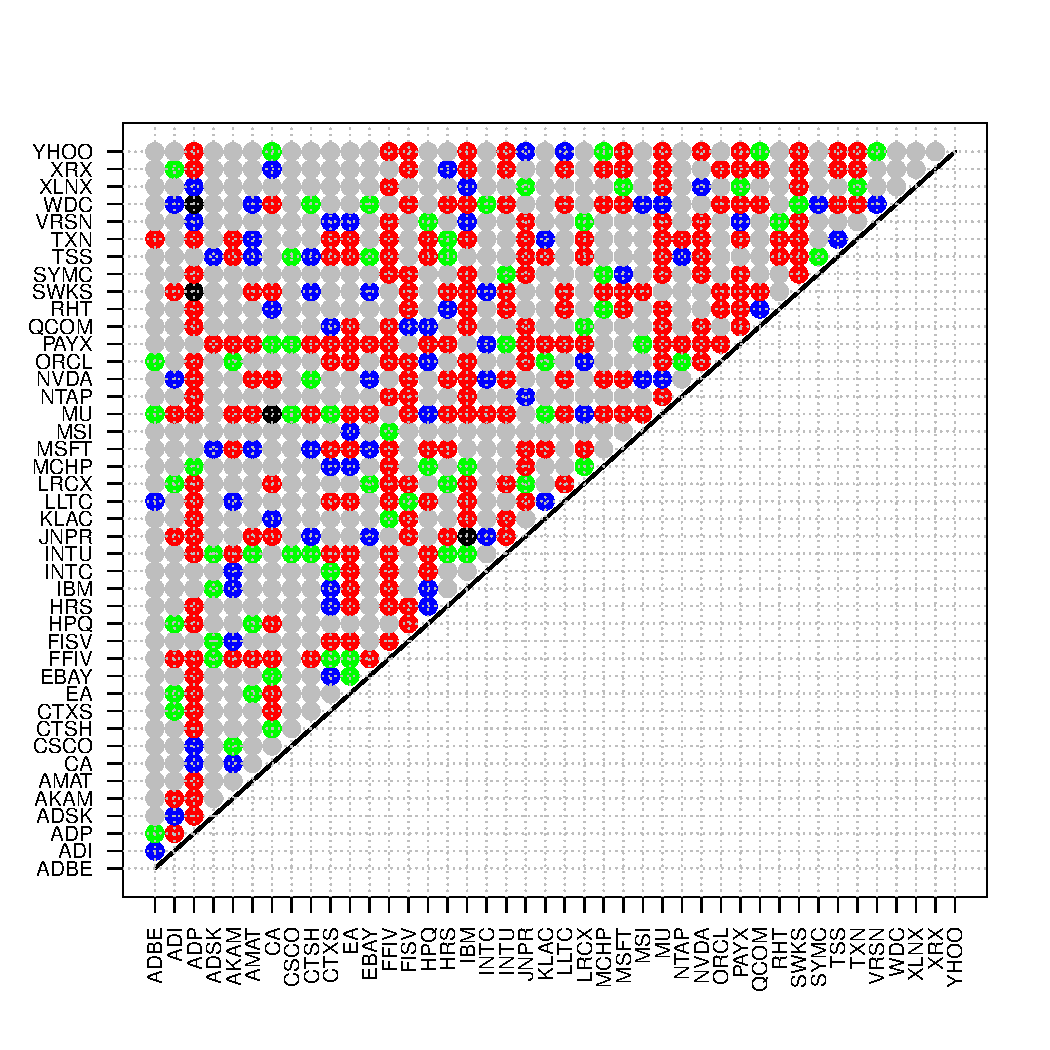
\includegraphics[
      width=\textwidth,
      trim={0.3cm, 0.8cm, 1cm, 0.6cm}, clip
    ]{Hoga_IT_pair_permuted.pdf}
  \end{minipage}
  \caption{
    Test for changing tail-index or scale parameter
    of losses
    using Hoga's test based on concatenated series of pairs of
    stocks.
    A random permutation is applied to the observations of each
    series.
    The green, blue and red points
    correspond to pairs of stock in a sector 
    when the test statistic $T_n$ exceeds the $85\%$-, $90\%$-,
    $95\%$-quantile of the limit \ds .
    Grey points stand for pairs for which the test statistic is below
    the \asy\ $85\%$-quantile. Black points represent 
    pairs for which the computation of $T_n$ fails for given precision  
    requirements and time limits.
  }
  \label{fig:PairTest:permuted} 
\end{figure}


\newpage
\section{Some theoretical arguments for equality of tail-indices}\setcounter{equation}{0}\label{sec:2}
\subsection{Multivariate GARCH models whose components have  equal tail-indices}\label{subsec:garch}
Among the models for returns the generalized autoregressive conditionally heteroscedastic (GARCH) model
is certainly most popular because it is parsimonious, captures various of the stylized facts of real return data
and can also be modified in various directions to capture specific behavior of \ts\ such a asymmetry, skewness, long memory; 
see for example Andersen et al. \cite{andersen:davis:kreiss:mikosch:2009}, Part 1, for a collection of results
on GARCH-type models.
The original  {\em univariate} GARCH model of Bollerslev \cite{bollerslev:1986} is a stochastic volatility model of the type $X_t=\sigma_t\,Z_t$, where 
$(Z_t)$ is an iid mean-zero unit-variance \seq . In the simple case of a GARCH the {\em squared volatility} satisfies the {\em stochastic recurrence equation} 
\beam\label{eq:5}
\sigma_t^2= \alpha_0+\alpha_1 X_{t-1}^2+\beta_1\sigma_{t-1}^2=\alpha_0+(\alpha_1Z_{t-1}^2+\beta_1)\sigma_{t-1}^2\,,\quad t\in\bbz\,.
\eeam
Here $\alpha_0>0$, $\alpha_1,\beta_1$ are non-negative constants. For suitable choices of $\alpha_1,\beta_1$ the equation \eqref{eq:5}
can be solved and the solution $(\sigma_t^2)$ constitutes a strictly stationary \seq , implying that $(X_t)$ 
is strictly stationary itself. A remarkable property of the process $(\sigma_t)$ is that it has a power-law tail 
of the form
\beam\label{eq:6}
\P(\sigma_t>x)\sim c\,x^{-\alpha}\,,\qquad \xto\,,
\eeam
for some positive $c>0$ and a positive tail-index $\alpha$ which is the unique solution of the equation 
$\E [(\alpha_1 Z_1^2+\beta_1)^{\alpha/2}]=1$
provided that the solution exists and some mild assumptions on the \ds\ of $Z_t$ hold. This result
follows by an application of the Kesten-Goldie theorem; see Kesten \cite{kesten:1973}, Goldie \cite{goldie:1991}, cf. 
Buraczewski et al. \cite{buraczewski:damek:mikosch:2016} for a 
recent textbook treatment. The latter result ensures power-law tails  for
the strictly stationary  solution $(Y_t)$ to the stochastic recurrence equation\ 
\beam\label{eq:7}
Y_t= A_t\,Y_{t-1}+B_t\,,\qquad t\in\bbz\,,
\eeam
for an iid \seq\ of pairs $(A_t,B_t)$, $t\in\bbz$, with non-negative components satisfying $\E [A_1^{\alpha/2}]=1$.  
In the model \eqref{eq:5} we can choose $Y_t=\sigma_t^2$, $A_t=\alpha_1\,Z_{t-1}^2+\beta_1$ and $B_t=\alpha_0$ to achieve
\eqref{eq:6}. In turn, by an application of Breiman's lemma (see \cite{buraczewski:damek:mikosch:2016}, p.~275)
it follows that
\beao
\P(\pm X_t>x)\sim \E[(Z_t)_\pm^\alpha]\,\P(\sigma_t>x)\,,\qquad \xto\,, 
\eeao
implying power-laws for the right and left tails of $X_t$ caused by the power-law tail of $\sigma_t$.

A GARCH process of the order $(p,q)$ can be embedded in a multivariate
equation of the type \eqref{eq:7}, where $(\bfA_t)$ are iid random
matrices and $\bfB=\bfB_t$ is a constant vector. Again, the Kesten
theory \cite{kesten:1973} applies, implying that the marginal and
\fidi s of the GARCH process are \regvary\ with a positive index
$\alpha$. We refrain from explaining the notion of multivariate
\regvar\ which is needed in this context. For further details, see
Buraczewski et al. \cite{buraczewski:damek:mikosch:2016} where the
Kesten theorem and \regvar\ of GARCH processes are explained in detail.
\par
There exist various extensions of the univariate GARCH
model to the multivariate case. For the sake of argument, we stick here to the 
{\em constant conditional correlation} (CCC) model of Bollerslev
\cite{bollerslev:1990} and Jeantheau \cite{jeantheau:1998}, and we only consider a special bivariate case.
It is the model 
\beao\bfX_t=
\left(\barr{l}X_{1,t}\\
X_{2,t}\earr\right)= \left(\barr{ll}\sigma_{1,t}& 0\\
0&\sigma_{2,t}\earr\right)\,\left(\barr{l}Z_{1,t}\\Z_{2,t}\earr\right)=\Sigma_t\,\bfZ_t\,,\qquad t\in\bbz\,.
\eeao
Thus both return components $X_{i,t}$ have the form of a univariate
stochastic volatility model $X_{i,t}=\sigma_{i,t}Z_{i,t}$ 
with non-negative volatility $\sigma_{i,t}$ and an iid bivariate noise \seq\ $(\bfZ_t)$ with zero mean and unit variance components.
We also have the specification
\beam\label{eq:8}
\bfY_t=\left(\barr{l}\sigma^2_{1,t}  \\  
\sigma^2_{2,t}\earr
\right)
&=& \left(
\barr{l}\alpha_{01}  \\\alpha_{02}   \earr\right)
+\left(\barr{cc}\alpha_{11} & \alpha_{12}  \\
      \alpha_{21} & \alpha_{22}\earr \right)\, 
\left(\barr{l}X_{1,t-1}^2  \\X_{2,t-1}^2   \earr\right)
 + \left(\barr{cc}\beta_{11} & \beta_{12}  \\\beta_{21} & \beta_{22} \earr
 \right)\,\left(\barr{c}\sigma^2_{1,t-1}  \\\sigma^2_{2,t-1}\earr
  \right)\nonumber\\
&=& \left(
\barr{l}\alpha_{01}  \\\alpha_{02}   \earr\right)+\left(\barr{cc}\alpha_{11}Z_{1,t-1}^2+\beta_{11}&\alpha_{12}Z_{2,t-1}^2+
\beta_{12}\\
\alpha_{21}Z_{1,t-1}^2+\beta_{21}& \alpha_{22}Z_{2,t-1}^2+\beta_{22}
\earr\right)\,\left(\barr{l}\sigma_{1,t-1}^2\\\sigma_{2,t-1}^2\earr
\right)\,,
\eeam
for positive $\alpha_{0i}$ and suitable non-negative 
$\alpha_{ij},\beta_{ij}$, $i,j=1,2$.
Writing
\beao
\bfB_t= \left(
\barr{l}\alpha_{01}  \\\alpha_{02}   \earr\right)\quad\mbox{and}\quad
\bfA_t=\left(\barr{cc}\alpha_{11}Z_{1,t-1}^2+\beta_{11}&\alpha_{12}Z_{2,t-1}^2+
\beta_{12}\\
\alpha_{21}Z_{1,t-1}^2+\beta_{21}& \alpha_{22}Z_{2,t-1}^2+\beta_{22}
\earr\right)\,,
\eeao
we see that we are again in the framework of a stochastic recurrence equation\ 
but this time for vector-valued $\bfB_t$ and matrix-valued $\bfA_t$:
\beam\label{eq:jan6b}
\bfY_t=\bfA_t\,\bfY_{t-1}+\bfB_t\,,\qquad t\in\bbz\,.
\eeam
Kesten \cite{kesten:1973} also provided the corresponding theory  
for stationarity and tails in this case. \sta\ \cite{starica:1999}
dealt with the corresponding problems for CCC-GARCH processes,
making use of the theory in Kesten \cite{kesten:1973},
Bougerol and Picard \cite{bougerol:picard:1992}
and its
specification to the tails of GARCH models 
in Basrak et al.~\cite{basrak:davis:mikosch:2002}. \sta\ \cite{starica:1999} assumed the 
Kesten conditions for the matrices $\bfA_t$. These conditions ensure that the product matrices $\bfA_1\cdots\bfA_n$ 
have positive entries for sufficiently large $n$. Then Kesten's theory implies that
all components of the vector $\bfX_t$ have power-law tails with the same index $\alpha$ and also
that the \fidi s of the process $(\bfX_t)$ are \regvary\ with index $\alpha$. 
\par
Various GARCH modifications are derived by considering linear combinations of CCC-GARCH models.
The property of multivariate \regvar\ of multivariate GARCH ensures that, after linear transformations,  
the new process in all components has again power-law tails with the same index as the original GARCH process; see 
Basrak et al.~\cite{basrak:davis:mikosch:2002}. 
Models which are constructed in this way are
the Orthogonal GARCH model of
Alexander and Chibumba \cite{alexander:chibumba:1996}, its
generalization GO-GARCH by van der Weide \cite{Weide2002},  the Full Factor GARCH model of Vrontos et al.
\cite{vrontos2003full} and the Generalized Orthogonal Factor GARCH
model of Lanne and Saikkonen  \cite{lanne2007modelling}. These
models are characterized by their treatment of each series as a linear
combination of factors, and each of the factors is modeled as a GARCH
process; see Silvennoinen and Ter\"asvirt\"a \cite{silventeras:2009}.
\par
Not all choices of $\alpha$- and $\beta$-parameters in the model \eqref{eq:8} allow for an
application of the Kesten theory. For example, assume that only the
diagonal elements $\alpha_{ii}$ and $\beta_{ii}$ are positive.
Then $\bfA_t$ is diagonal and, hence, the condition that
$\bfA_1\cdots\bfA_n$ have positive entries for sufficiently large $n$ 
cannot be satisfied. In the latter situation, both $(X_{1,t})$ and
$(X_{2,t})$ are univariate GARCH processes. Assuming the 
conditions of the univariate Kesten-Goldie theorem for each component
process, $(X_{1,t})$ and $(X_{2,t})$ have power-law tails 
with indices $\kappa_1$ and $\kappa_2$, respectively,  given by the solutions to the equations 
$\E [(\alpha_{ii} Z_{i,t}^2+\beta_{ii})^{\kappa_i/2}]=1$, $i=1,2$. In
this model, one can introduce dependence between the two component
series $(X_{1,t})$ and $(X_{2,t})$ by assuming dependence between the
noise variables $Z_{1,t}$ and $Z_{2,t}$. Another situation when the
Kesten theory fails 
appears when $\bfA_t$ is an upper or lower triangle matrix: then the
products  $\bfA_1\cdots\bfA_n$ are always of the same triangular
type. 
Similar remarks apply when one considers a CCC model in general
dimension. Of course, one may argue that the latter models 
are not natural: they are degenerate since they do not allow 
for a linear relationship
between all squared volatilities on a given day. 

\subsection{A utility based argument for equal tail-indices}\label{sec:3}
In this section we give an argument based on economic theory that
suggests equality of  tail-indices for equity return series.
We follow an approach by Routledge and Zin
\cite{routledge2010generalized} who introduced the notion of
Generalized Disappointment Aversion (GDA). We consider the risky
payoff $C$ of an investor and assume that it has a continuous \ds\ on
$(0,\infty)$ with distribution function $F_C$. Let $u$ be a utility \fct\ assumed to be
increasing and concave on $(0,\infty)$.  Following Routledge and Zin
\cite{routledge2010generalized},
the utility of an agent with GDA preferences is given by
\beao% \label{eq:xxie0}
  \wt u&=& \E [u(C)] - b\, \int_{0}^{\delta v}
  \big[ u(\delta \,v) - u(x) \big] F_C(dx)\,,
  %&=&
  %\E u(C) - b \E\big[\big(u(\delta \,v) - u(C)\big)\1( C \le  \delta \,v)\big]\,,
\eeao
where $\delta $ and $v$ are positive constants, and $b\ge 0$.
  Here $v$ can be thought of as the {\em certainty payoff} equivalent to the
 risky payoff $C$; $\delta$ tunes the {\em threshold of 
   disappointment} in proportion to $v$; $b$ determines the extra
 weight given to the expected return of $C$ when $C$ is below the
 disappointment threshold $\delta v$.
 If $b=0$, preferences are the classical expected utility. If
 $\delta=1$ and $b>0$ preferences follow Gul's \cite{gul:1991} 
disappointment aversion which were generalized by Routledge and Zin
\cite{routledge2010generalized}.
\par
An agent guided by the utility function $u$ will seek to maximize the
\fct al $\wt u$.
Routledge and Zin assumed a power-law utility function 
\beam\label{eq:hjyr}
u(x)=-\frac{1}{\xi}\,x^{-\xi}\,,\quad \xi>0\,. 
\eeam

For the sake of argument, we assume that an investor initially has one
unit of wealth. He invests $1-\phi\in (0,1)$ units in a risk-free 
bond with interest rate $r>0$ and $\phi$ units in a risky asset with
return $X$ over one time unit, i.e.,
\beam\label{eq:xxie1}
  C(X) = (1 - \phi)\, \ex^{r} + \phi \,\ex^{X}\,.
\eeam
Then we have 
\beao
\wt u(F_X, \phi) &=& \E [u(C)] + b\, \E \big[u(C)\1(C \le  \delta v)\big] - b \,u(\delta\, v) F_X(q)\,,
\eeao
where $F_X$ is the distribution function of $X$  and
\beao
  q = %q(r, \phi) &:=& \log \left( {
      %\delta v - (1 - \phi) e^r
      %\over
      %\phi
    % \right) 
\log\Big(
    \ex^r + {\delta \,v - \ex^r \over \phi}
  \Big)\,.
\eeao
Note that $C \le \delta v$ \fif\ $X \le  q$. 
\par
Naturally, if an agent invests in
a risky asset instead of a riskless bond, he expects to obtain a
higher (on average) return from the risky asset than he is guaranteed from the
riskless bond. In our notation, this means $\delta \,v > \ex^r$ or
$q > r $. For given $b,\delta,v$, the \fct al $\wt u$  depends only on $\phi$ and $F_X$,
$\wt u=\wt u (F_X, \phi)$.
We assume that
\beao
\wt u_{\rm max}=\wt u_{\rm max}(F_X) = \max_{0 \le  \phi \leq 1} \wt u (F_X,\phi)
\eeao
exists and that the maximum is achieved at a unique $\hat\phi \in (0, 1)$.

\subsection{Pareto-distributed returns}\label{sec:pareto_tail}
Since we are interested in the influence of heavy-tailed losses on the preferences of an investor 
we assume the following toy model. 
We consider the case when $X$ has a two-sided Pareto \ds\ given by
\beam\label{eq:pareto}
  F_X(x) = \left\{
  \begin{array}{ll}
    p \left(
    {K \over K - x}
    \right)^\alpha & x \leq 0 \,,\\
    1 - (1 - p) \left(
    {K' \over K' + x}
    \right)^\beta & x > 0\,,
  \end{array}
  \right.
\eeam
where
$\alpha, \beta > 0$, $K,K' > 0$, $0 < p < 1$. 
We also write $f_X$ for the density function of $F_X$.
\par
We have
\beam\label{eq:xxie1.0}
 \wt u(F_X, \phi)\nonumber
  &=&
  \alpha\, K^\alpha\,  p\,
  \int_{-\infty}^0
  u\big( (1 - \phi) \ex^r + \phi \ex^x \big)\,
  {1 + b \over (K - x)^{\alpha + 1}} \,dx\\
    &&+
  \beta \,(K')^\beta\, (1 - p)
  \int_{0}^\infty
  u\big( (1 - \phi) \ex^r + \phi\, \ex^x \big)\,
  {1 + b \1(x <  q) \over (K' + x)^{\beta + 1}} \,dx 
  - b \,u(\delta v) \,F_X(q) \,.\label{eq:pp}
\eeam
\par
We observe the following property 
whose proof is given in Appendix~\ref{sec:thrmI_proof}. 
% which also applies to the special case 
%\eqref{eq:xxie1.0}. 
\ble\label{thrm:I}
Assume the two-sided Pareto model \eqref{eq:pareto},
that there is no \fct al relationship between $\alpha,K$ and $\beta,K'$
and the utility \fct\ $u$ is increasing and differentiable. Then
$\frac{\pd \wt u_{\rm max}}{\pd \alpha} > 0$ and
$\frac{\pd \wt u_{\rm max}}{\pd K} < 0$.
\ele
We conclude that
$\wt u_{\rm max}$ increases with $\alpha$ and decreases with
$K$. Therefore there is a curve of  equal preference on the $(\alpha,
K)$-plane. Moving along this curve in the direction of increasing
$\alpha$, one expects the values of $K$ to increase too, i.e., the
estimated values of $\alpha$ and $K$ 
should appear positively dependent. Figure~\ref{fig:preference_pareto}
illustrates this scenario for $\xi = 1/2, 4$ for the power-utility
\fct\ \eqref{eq:hjyr}.
In fact, this positive dependence is indeed observed for some
real return data, e.g. the ``Energy'', ``Consumer Staples'' and
``Information Technology'' sectors of the S\&P 500 index; see 
Figure~\ref{fig:sectors_parameters}.
\par
A particularly interesting case occurs  when 
$F_X$ is symmetric, i.e., when $\alpha = \beta$, $K =K'$ and $p=0.5$.
Then \eqref{eq:pareto} turns into 
\begin{eqnarray}
  \wt u(F_X, \phi) &=& {\alpha \over 2} K^\alpha (1 + b)
  \int_{0}^\infty {
    u(C(x)) \left[
      1 - {b \over 1 + b}\1_{\{x \ge q\}}
      \right]
    + u(C(-x))
    \over
    (K + x)^{\alpha + 1}
  } dx
  - b u(\delta v) F_X(q)\,.\nonumber\\
  \label{eq:ipf}
\end{eqnarray} 
This situation is not covered by Lemma~\ref{thrm:I}:
for the proof of the latter result we used Lemma \ref{lemma:I} whose
assumptions are not satisfied in the present situation.
Indeed, the integrand 
\[
U_{\text{all}}(x) =
u(C(x)) \left[
  1 - {b \over 1 + b}\1(x \ge q)
  \right]
+ u(C(-x))
\]
is not monotone.\footnote{To see this we may plug \eqref{eq:hjyr} 
in $U_{\text{all}}$ and re-write it as
\[U_{\text{all}}(x) =
  -{\phi^{-\xi} \over \xi} \Big\{
  \underbrace{
    \Big(1 - {b \over 1 + b}\1(x \ge q)\Big)
    \big[a + e^x\big]^{-\xi}
    +
    \Big[a + e^{-x}\Big]^{-\xi}
  }_{U(x)} \Big\}\,,
\]
where $a = (1 - \phi) e^r/\phi$.
Direct computation gives
\begin{eqnarray*}
  U'(x)
  &=&
  -{(a + e^x)^{-\xi - 1} \xi e^x
    \over
    1 + b \1(x \ge  q)
  } + (a + e^{-x})^{-\xi - 1} \xi e^{-x}\,,
  \qquad x \neq q
\end{eqnarray*} 
The \fct\ $U(x)$, hence $U_{\text{all}}$, 
is not monotone because $U'(x)>0$ for all large $x$ while $U(x)$ decreases
in a small neighborhood of $q$.}
\par
We resort to numerical methods to gain some understanding of
how $\tilde u(F_X, \phi)$ changes with $\alpha$.
The value of $\hat\phi$ can be calculated
by numerical integration and optimization with respect to $\phi$ for
given values of $K, K', \alpha, \beta$.  This is shown in 
Figure~\ref{fig:phi_hat_pareto} for the power utility \fct\
\eqref{eq:hjyr} both for fixed $K', \beta$ and for $K=K'$, $\alpha=\beta$.  
The corresponding values $\tilde u_{\rm max}(\alpha, K)$
are shown in Figure \ref{fig:preference_pareto}.
If $K'$ and $\beta$ are fixed, both $\wt u_{\rm max}(\alpha, K)$ 
and $\hat\phi$ increase  with $\alpha$ and decrease with $K$. 
This is in agreement with Lemma~\ref{thrm:I}. 
In contrast, when $K=K'$ and $\alpha=\beta$
$\wt u_{\rm max}(\alpha, K)$ decreases with $\alpha$ 
but is rather insensitive with respect to $K$. On the
other hand, $\hat\phi$ is not monotone with respect to $\alpha$ or
$K$. For each fixed $K$, it peaks at an $\alpha$-value somewhere below
1. For realistic values $\alpha\in (2, 4)$, $\hat\phi$ is a
small value below 5\%.
Since $\wt u_{\rm max}(\alpha, K)$ decreases with
$\alpha$, investors who seek to maximize $\wt u_{\rm max}(\alpha, K)$
will prefer the smallest $\alpha$ in the market, resulting in similar
values of $\alpha$ for different equities.
\begin{figure}[htb!]
  \begin{minipage}{0.25\linewidth}
    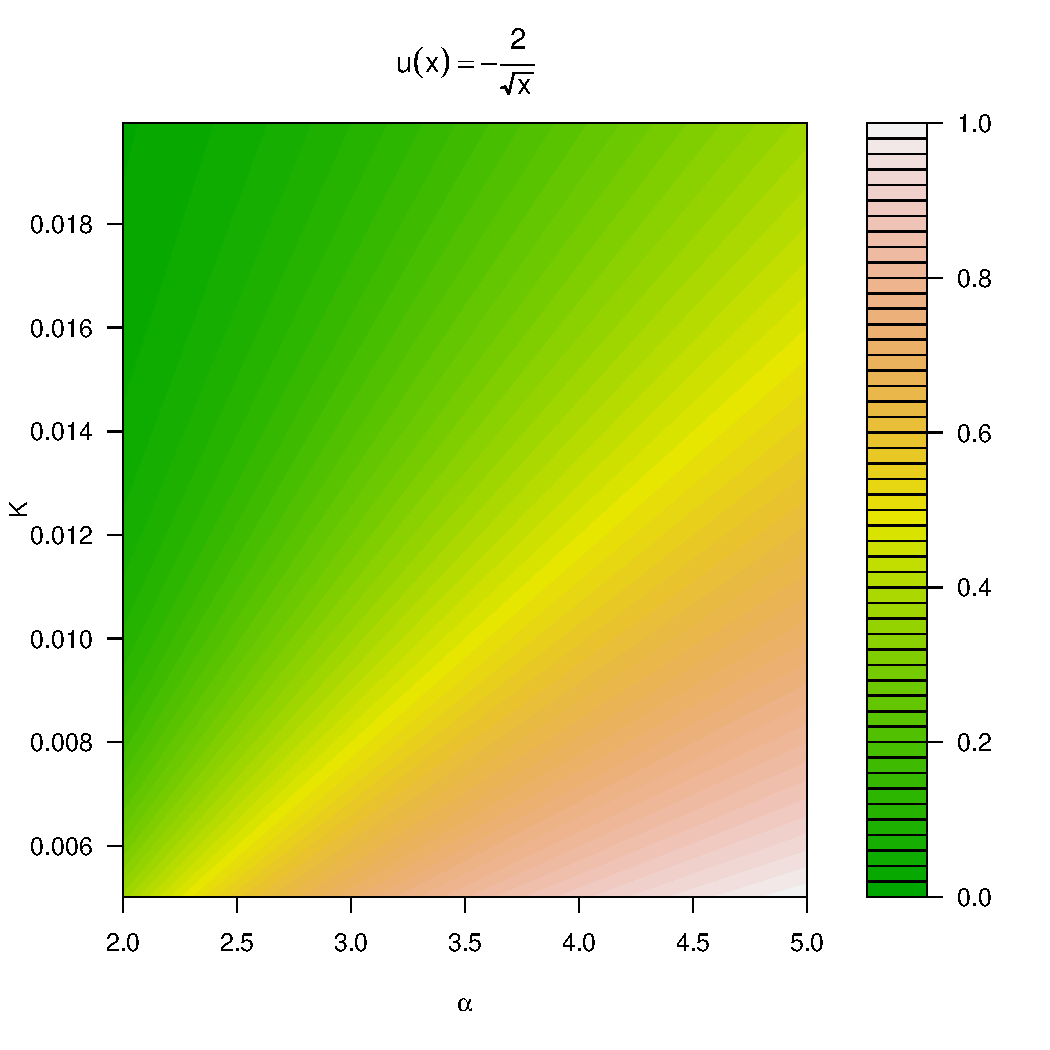
\includegraphics[width=\textwidth]{phi_hat_pareto5e-1_A.pdf}    
  \end{minipage}\hfill
  \begin{minipage}{0.25\linewidth}
    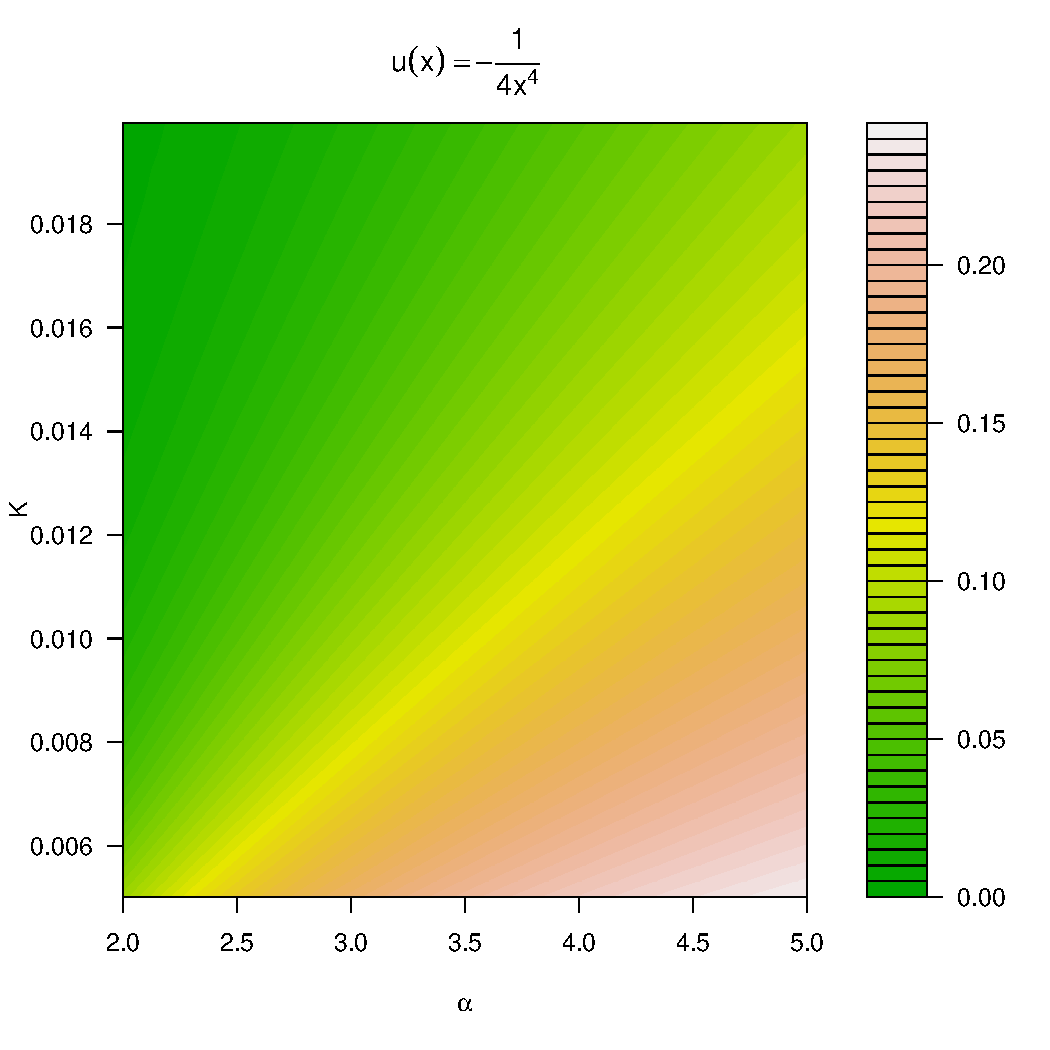
\includegraphics[width=\textwidth]{phi_hat_pareto4_A.pdf}
  \end{minipage}\hfill
  \begin{minipage}{0.25\linewidth}
    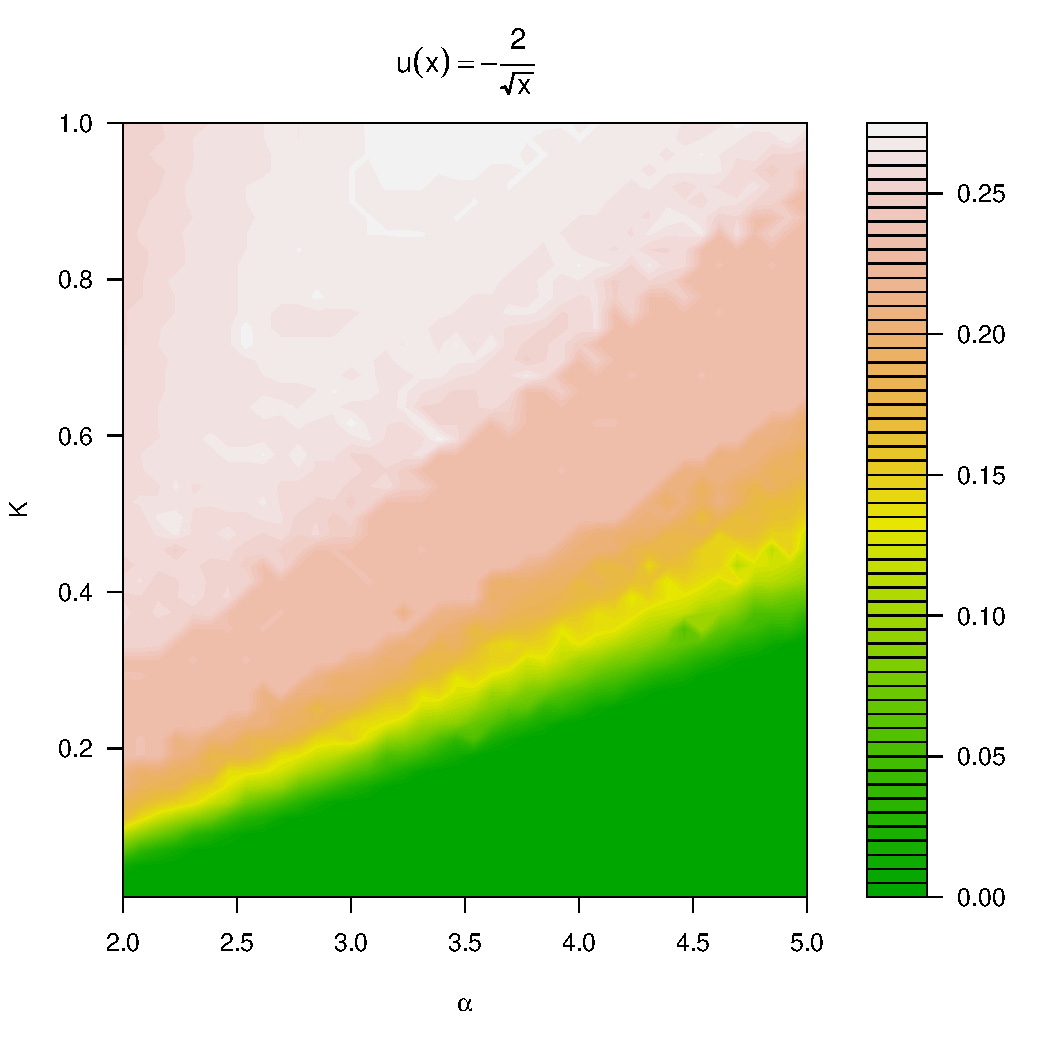
\includegraphics[width=\textwidth]{phi_hat_pareto5e-1.pdf}    
  \end{minipage}\hfill
  \begin{minipage}{0.25\linewidth}
    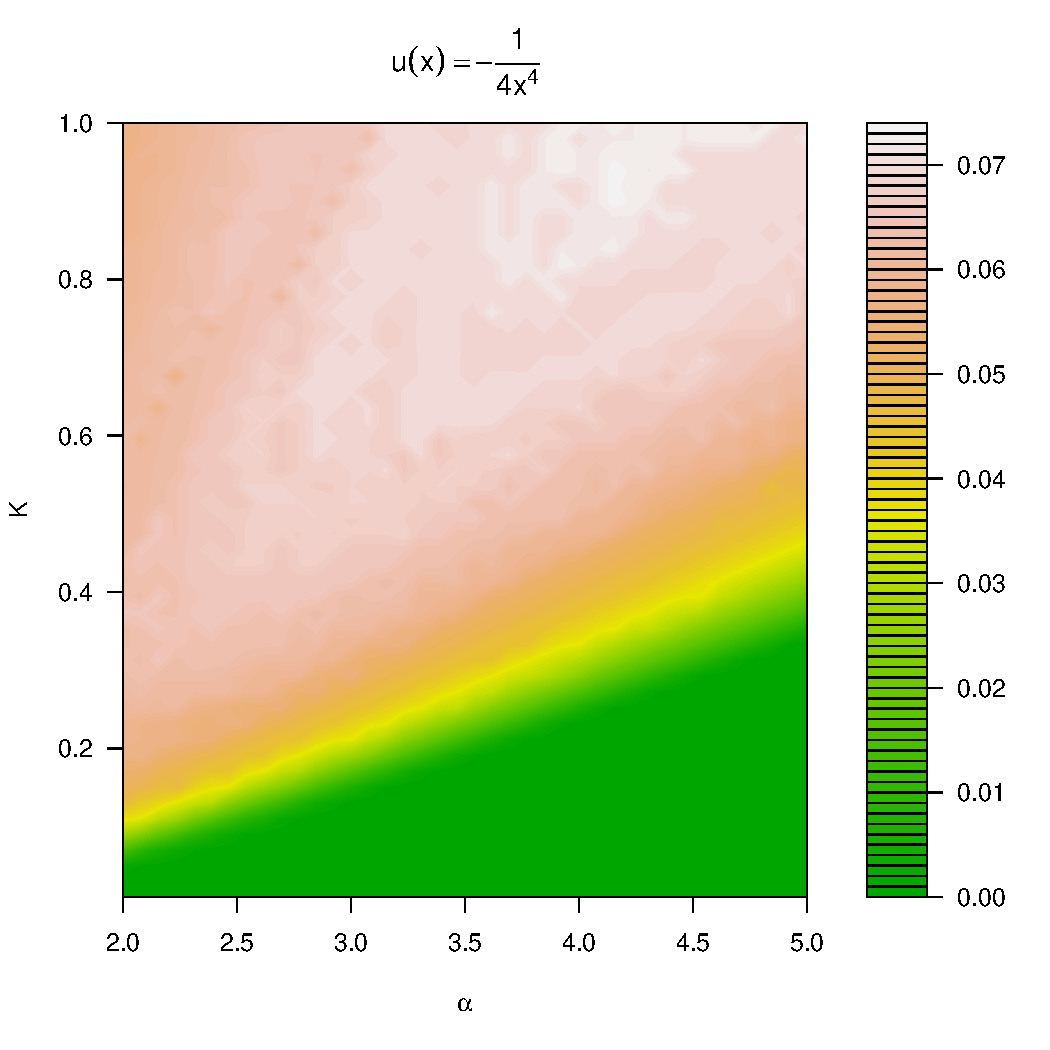
\includegraphics[width=\textwidth]{phi_hat_pareto4.pdf}
  \end{minipage}
 \caption{
   {\em The 1st and 2nd} graphs show $\hat\phi$, the optimal equity
   allocation as a \fct\ of $\alpha$ and $K$ in the two-sided Pareto model
   \eqref{eq:pareto} for fixed $K'=0.012$, $\beta = 1.4$.
   {\em The 3rd and 4th} graphs show $\hat\phi$ as a \fct\ of $\alpha$
   and $K$ with $\beta = \alpha$ and $K' = K$.
   We choose the utility \fct\ $u$ from \eqref{eq:hjyr} for $\xi = 1/2$
   and $\xi = 4$, $b = 0.01$ in all cases.
  }
  \label{fig:phi_hat_pareto}
\end{figure}

\begin{minipage}{0.5\linewidth}
  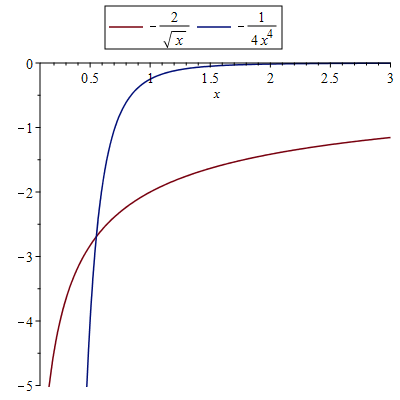
\includegraphics[width=\textwidth]{power_utilities.png}
\end{minipage}\hfill
\begin{minipage}{0.42\textwidth}
  The economitrical differences between the two utility functions
  are illustrated in the graph to the left.
  We see that
  $u(x)$ grows slower and saturates later for small $\xi$ than for
  large $\xi$. The latter case represents an agent who is more
  tolerant about low consumption and seeks wealth more
  aggressively. In other words, he is less risk-averse than one with a
  larger $\xi$. Such an agent will therefore invest more heavily in
  equity, as shown in Figure~\ref{fig:phi_hat_pareto}. Note that,
  while $\hat \phi$ changes nearly in the same in both graphs, the
  scales in the graphcs are very different.
\end{minipage}

\begin{figure}[htb!]
  \begin{minipage}{0.25\linewidth}
    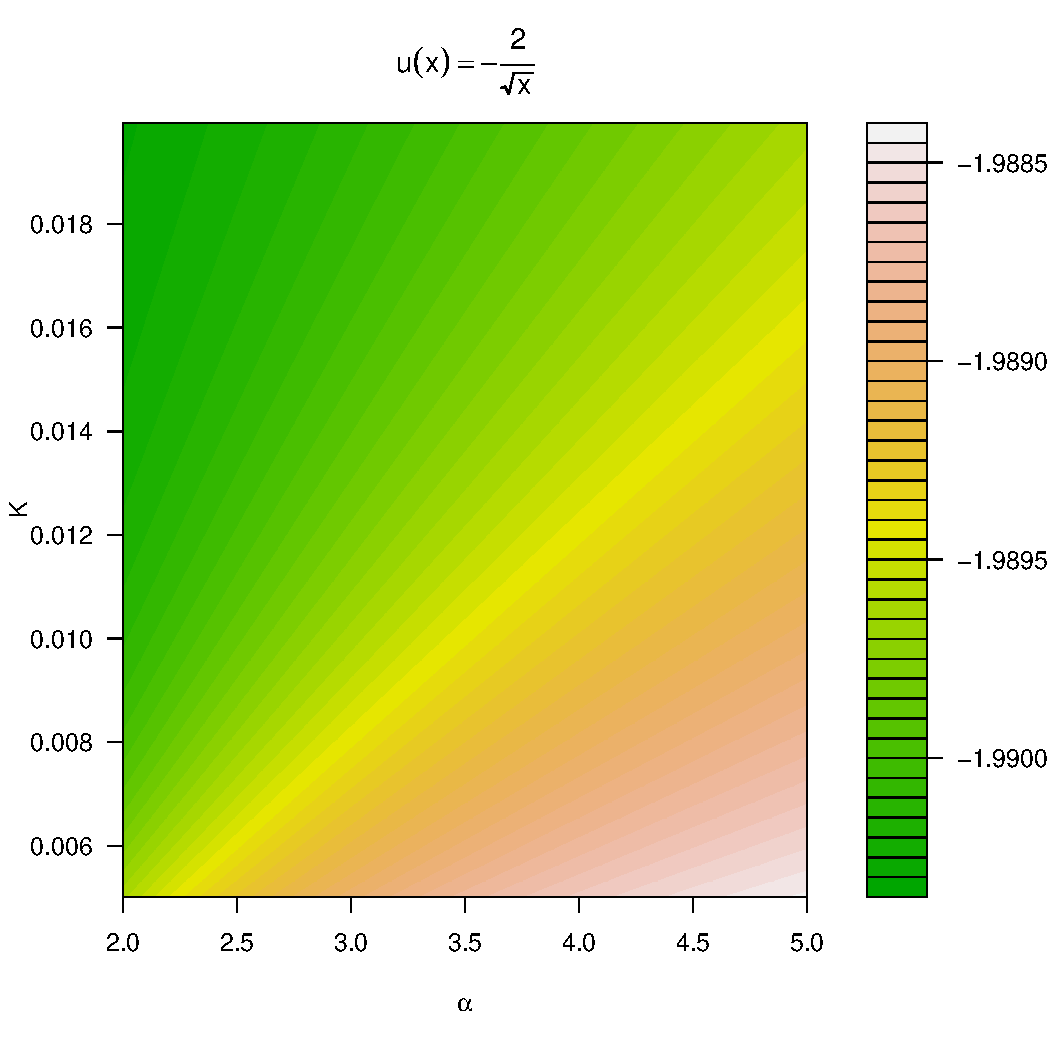
\includegraphics[width=\textwidth]{preference_pareto5e-1_A.pdf}
  \end{minipage}\hfill
  \begin{minipage}{0.25\linewidth}
    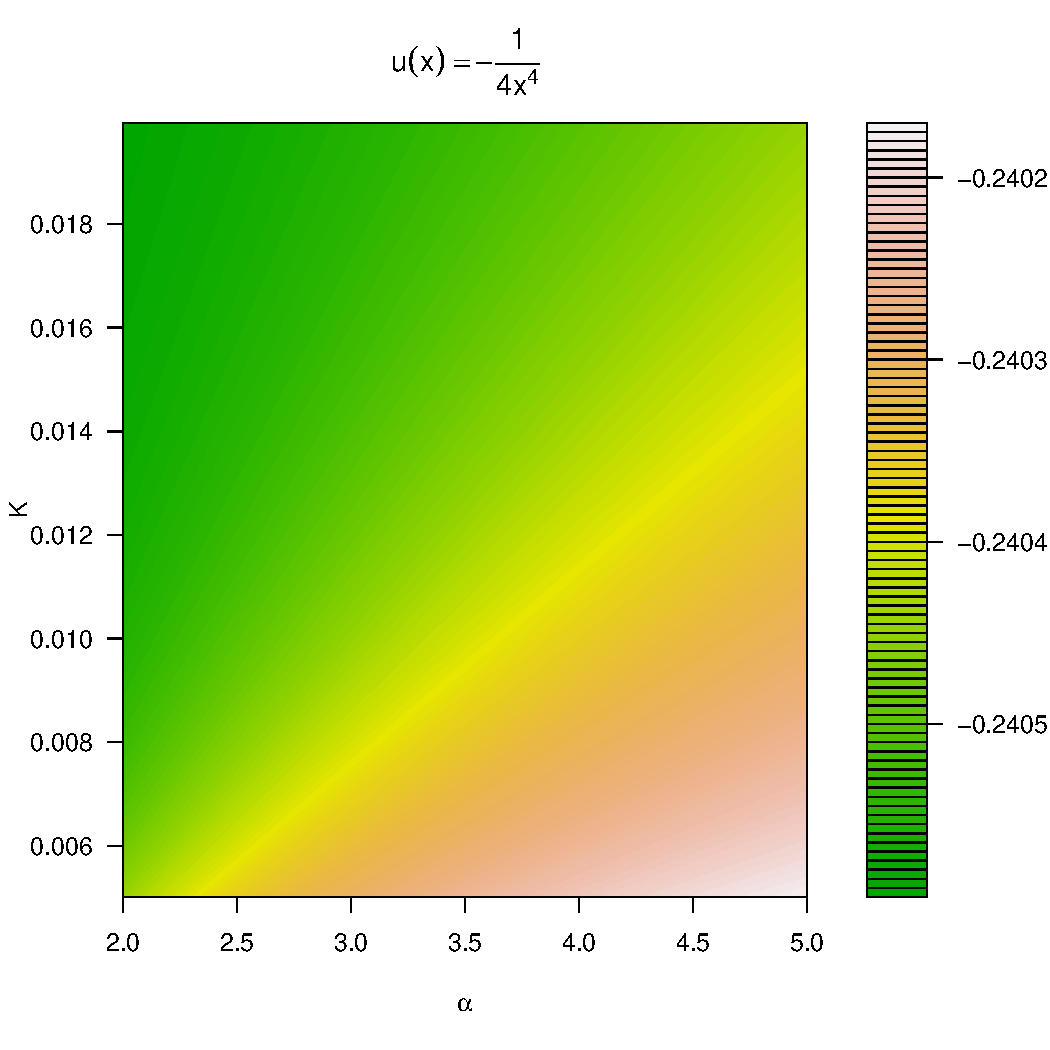
\includegraphics[width=\textwidth]{preference_pareto4_A.pdf}
  \end{minipage}\hfill
  \begin{minipage}{0.25\linewidth}
    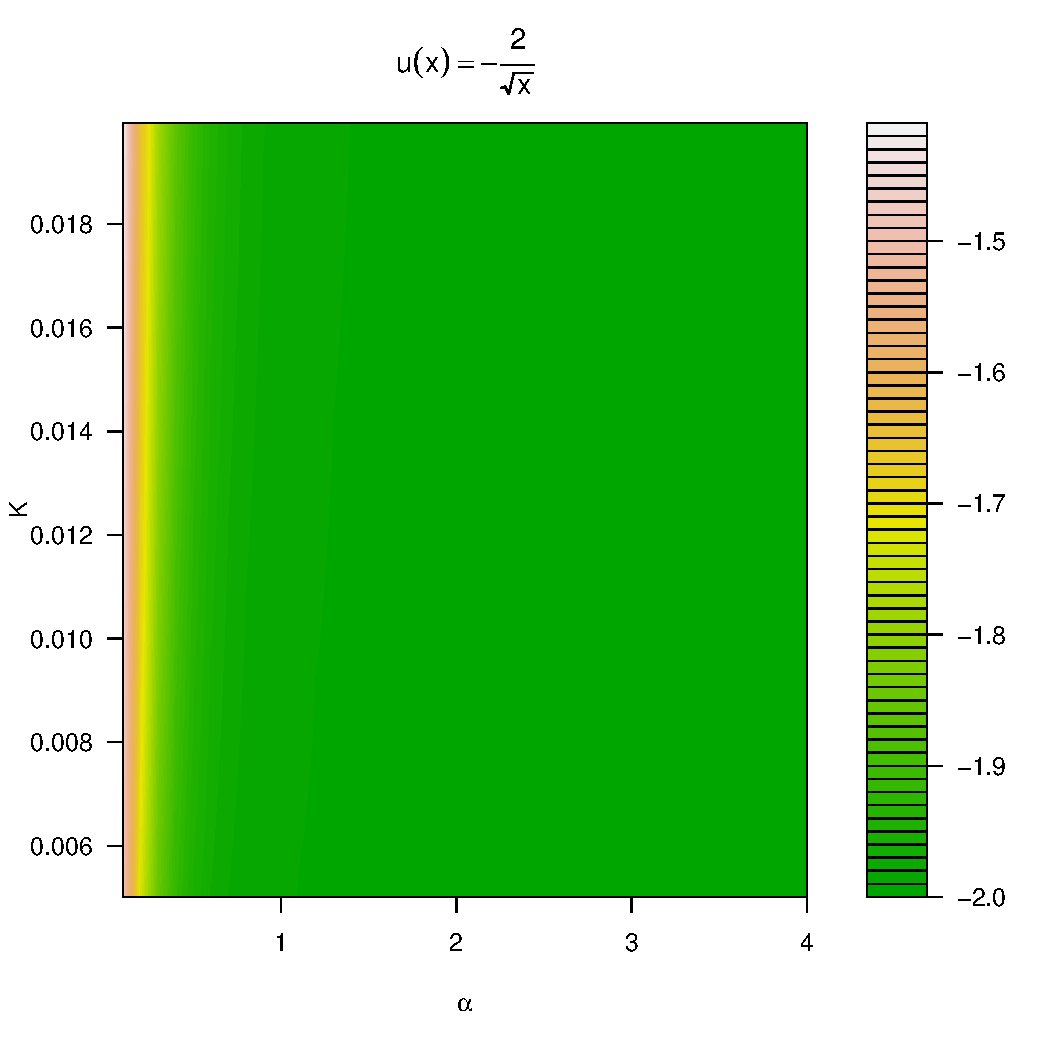
\includegraphics[width=\textwidth]{preference_pareto5e-1.pdf}
  \end{minipage}\hfill
  \begin{minipage}{0.25\linewidth}
    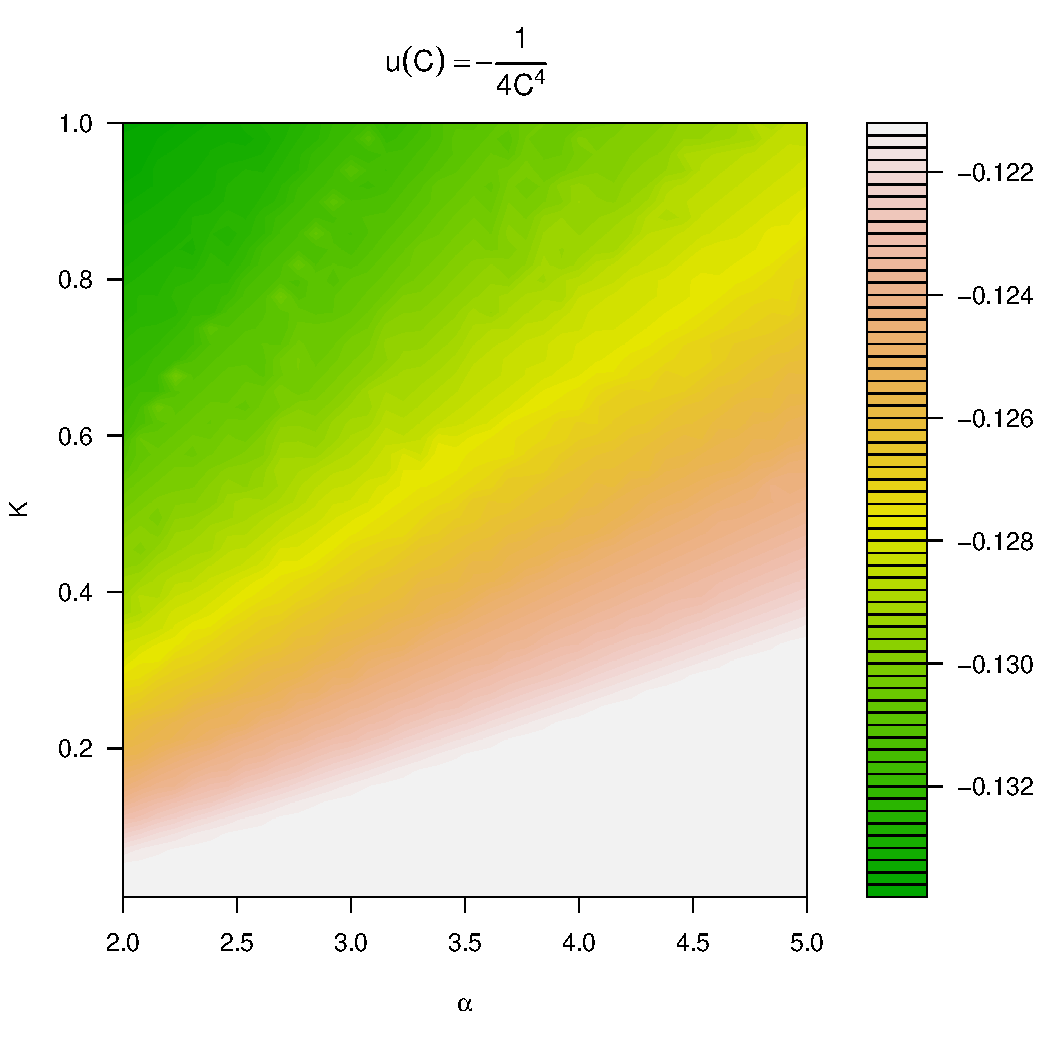
\includegraphics[width=\textwidth]{preference_pareto4.pdf}
  \end{minipage}
  \caption{
   {\em The 1st and 2nd} graphs show
   $\tilde u_{\rm max}(\alpha, K)$, as a \fct\ of $\alpha$ and $K$
   in the two-sided Pareto model \eqref{eq:pareto} with $K'=0.012$,
   $\beta = 1.4$.
   Clearly, $\tilde u_{\rm max}(\alpha, K)$ increases with $\alpha$
   and decreases with $K$ when $K'$ and $\beta$ are fixed.
   {\em The 3rd and 4th} graphs show
   $\tilde u_{\rm max}(\alpha, K)$ as a \fct\ of $\alpha$
   and $K$ with $\beta = \alpha$ and $K' = K$.
   We choose the utility \fct\ $u$ from \eqref{eq:hjyr} for $\xi = 1/2$
   and $\xi = 4$. $b = 0.01$ in all cases.
  }
  \label{fig:preference_pareto}
\end{figure}

If the parameter $b$ is very small the GDA preference is closely
approximated by the mean-utility preference, corresponding to $b = 0$. 
In this case, we show in the proof of Lemma \ref{lemma:III} that the function
$U_{\text{all}}(x)$ may increase or decrease depending on particular conditions
on the values of $\xi$ and $(1 - \phi) e^r / \phi$:
\begin{enumerate}
\item If $\max\{a, 1\} < \xi$, $U_{\text{all}}(\cdot)$ is
  monotone decreasing.
\item If $a < \xi < 1$ and $(a + y_-)/(a y_- + 1) <
  y_-^{(1-\xi)/(1+\xi)}$, $U_{\text{all}}(\cdot)$ is monotone
  decreasing.
\item If $\xi < a < 1$, $U_{\text{all}}(\cdot)$ is monotone
  increasing.
\item If $1 < \xi < a$ and $(a + y_+)/(a y_+ + 1) >
  y_+^{(1-\xi)/(1+\xi)}$, $U_{\text{all}}(\cdot)$ is monotone
  increasing.
\item In other case, $U_{\text{all}}(\cdot)$ is not monotone.
\end{enumerate}
where
\begin{eqnarray*}
a &=& {
  (1 - \phi) e^r
  \over
  \phi
} \\
y_\pm &=& {
  a^2 - \xi \pm \sqrt{(a^2 - 1) (a^2 - \xi^2)}
  \over
  a (\xi - 1)
}
\end{eqnarray*}
Moreover, it is also easily checked that, when
$x \in (0, K(e^{1/\alpha} - 1)]$,
the density function in the integral of \eqref{eq:ipf} increases
with $\alpha$; when $x \in (K(e^{1/\alpha} - 1), \infty)$ it 
decreases with $\alpha$. Following the arguments for Lemma~\ref{thrm:I},
and applying Lemma \ref{lemma:I}, it can be seen that
$\wt u_{\rm max}(\alpha, K)$ increases/decreases with $\alpha$ when
$U_{\text{all}}(x)$  decreases/increases.

\section{Conclusion}
\label{sec:4}
We have established that, in the case of an equity return series with
two-sided, functionally independent Pareto tails, investor
preference functionals are monotone increasing/decreasing with the
tail index/scale parameters. Thus in a market dominated by such
equities, the investors would pursue the largest tail index in the
market, leading to a shared common tail index for all equities.

The empirical results presented in section \ref{sec:1} suggest this
may well be the case for the ``Consumer Staples'' sector of S\&P 500,
given the Hill estimates of tail indices shown in figure \ref{fig:1}
and the largely positive results of tests for equal tail indices shown
in figure \ref{fig:PairTest}.

On the other hand, we have also seen that, when the left and the right
tails have the same indices, investor preference over the equity has
more sophisticated variations in the parameters' space including the
tail parameters of the equity, the interest rate, the investor's risk
apetite as captured by his utility function, and his threshold of
disappointment.

We also acknowledge that our model of the market and the investor is a
simple one, not accoounting for the dependence between equities, nor
the categorization of investors and their interactions. These are
potential topics of future work.

\ifx\phdthesis\undefined
\appendix
\else
\begin{subappendices}
\fi

\section{A monotonicity lemma}
\setcounter{equation}{0}
\begin{lemma} \label{lemma:I}
  Assume distribution function $F(x, \theta)$ parameterized by 
  $\theta \in \Theta \subseteq \mathbb R$ has support
  $(a, b) \subseteq \mathbb R$,
  and in addition $F(x, \theta)$ has density
  function $f(x, \theta)$ that is differentiable with respect to
  $\theta$ for all $\theta \in \Theta$.
  Let $X \sim F$ and assume function $h(\cdot)$ is defined on $(a, b)$
  and is monotone throughout this interval.
  Moreover, we assume $h(x)$ and $f(x, \theta)$ satisfy
  \begin{equation}\label{eq:frt}
%    \E |h(X)| < \infty, \quad
    \int_a^b \left| {\pd f(x, \theta) \over \pd \theta} \right| dx
    < \infty \text { and }
    \int_a^b \left| h(x) {\pd f(x, \theta) \over \pd \theta} \right| dx
    < \infty
  \end{equation}
  Then the following holds true:
  \begin{enumerate}
  \item If $h(\cdot)$ is decreasing and $\exists x_0 \in (a, b)$ such that
    $\frac{\pd f}{\pd \theta}(x, \theta) > 0$ for $x \in (a, x_0)$ while
    $\frac{\pd f}{\pd \theta}(x, \theta) < 0$ for $x \in (x_0, b)$, then
    \[
    \frac{\pd \E h(X)}{\pd \theta} > 0
    \]
  \item If $h(\cdot)$ is increasing and $\exists x_0 \in (a, b)$ such that 
    $\frac{\pd f}{\pd \theta}(x, \theta) < 0$ for $x \in (a, x_0)$  while
    $\frac{\pd f}{\pd \theta}(x, \theta) > 0$ for $x \in (x_0, b)$, then
    \[
    \frac{\pd \E h(X)}{\pd \theta} > 0
    \]
  \end{enumerate}
\end{lemma}
\begin{remark}
  \label{remark:I}
  Two other cases follow trivially from lemma \ref{lemma:I}:
  \begin{enumerate}
  \item If $h(\cdot)$ is increasing and $\frac{\pd f}{\pd \theta}$
    satisfies the
    same conditions of the 1st case of lemma \ref{lemma:I},
    $\frac{\pd \E h(X)}{\pd \theta} < 0$. This immediately follows
    from applying 1st case of lemma \ref{lemma:I} to $-h(\cdot)$.
  \item By the same argument, if $h(\cdot)$ is decreasing and
    ${\pd f \over \pd \theta}$ satisfies the same conditions of the
    2nd case of lemma \ref{lemma:I}, ${\pd \E h(X) \over \pd \theta} < 0$.
  \end{enumerate}
\end{remark}

\begin{proof}
  Firstly, by dominated convergence theorem, conditions \eqref{eq:frt}
  imply, for all $S \subseteq (a, b)$,
  \begin{eqnarray*}
    {\pd \over \pd \theta}\int_S f(x, \theta) dx
    &=&
    \int_S {\pd \over \pd \theta} f(x, \theta) dx \\
    {\pd \over \pd \theta}\int_S h(x) f(x, \theta) dx
    &=&
    \int_S h(x) {\pd \over \pd \theta} f(x, \theta) dx \\
  \end{eqnarray*}
  Thus we have
  \begin{eqnarray*}
    {\pd \E h(X) \over \pd \theta}
    &=&
    {\pd \over \pd \theta}
    \int_a^b h(x)
    f(x, \theta) dx \\
    &=& \int_a^b h(x)
    {\pd f \over \pd \theta}(x, \theta) dx \\
    &=& \underbrace{\int_a^{x_0}
      h(x) {\pd f \over \pd \theta}(x, \theta) dx}_{I_1}
    + \underbrace{\int_{x_0}^b
      h(x) {\pd f \over \pd \theta}(x,
      \theta) dx}_{I_2}
  \end{eqnarray*}
  $x_0$ being located in the interior of $(a, b)$ and
  $h(\cdot)$ being monotone imply $h(x_0) < \infty$.
  \begin{enumerate}
  \item When $h(x)$ is decreasing on $(a, b)$ and ${\pd f \over \pd
    \theta}(x, \theta) > 0$ on $(a, x_0)$
    \[
    I_1 > h(x_0) \int_a^{x_0}
    {\pd f \over \pd \theta}(x, \theta) dx
    \]
    Similarly, because ${\pd f \over \pd \theta}(x, \theta) < 0$ for
    $x \in (x_0, b)$ and $h(x)$ is decreasing, we have
    \begin{eqnarray*}
      I_2 &=& \int_{x_0}^b -h(x_0)
      \left|{\pd f \over \pd \theta}(x, \theta) \right| dx
      > -h(x_0)
      \int_{x_0}^b \left| 
        {\pd f \over \pd \theta}(x, \theta)
      \right| dx
    \end{eqnarray*}
    Finally we have
    \begin{eqnarray*}
      {\pd \E h(X) \over \pd \theta}
      > h(x_0) \int_a^b
      {\pd f \over \pd \theta}(x, \theta) dx
      = h(x_0) {\partial \over \partial \theta}
      \int_a^b f(x, \theta) dx
      = 0
    \end{eqnarray*}
  \item If $h(\cdot)$ is increasing and $\exists x_0 \in (a, b)$ such that 
    ${\pd f \over \pd \theta}(x_0, \theta) < 0$ on $(a, x_0)$  while
    ${\pd f \over \pd \theta}(x_0, \theta) > 0$ on $(x_0, b)$, 
    by similar arguments, one can show
    \[
    {\pd \E h(X) \over \pd \theta}> 0
    \]
\end{enumerate}
\end{proof}

\section{When equity returns follow Student's t-distribution}
\setcounter{equation}{0}
It is a common practice to use Student's t-distribution to model the
stationary distribution of equity returns. So it is of interest to
find out what implications this distribution has when it is combined
with the PDA preference. Formally we assume
\[
f(x; \alpha) = c(\alpha) \left(
  1 + {x^2 \over \alpha}
\right)^{-(\alpha + 1)/2}
\]
where $\alpha > 1$ and
\[
c(\alpha) = {
  \Gamma({\alpha + 1 \over 2})
  \over
  \Gamma(\alpha/2) \sqrt{\alpha \pi}
}
\]
In the same way as for \eqref{eq:ipf}, we can write $\wt u(F, \phi)$
as
\begin{small}
  \begin{eqnarray}
    \wt u(F, \phi)
    &=&
    (1 + b)
    \int_{0}^{\infty}
    \underbrace{
      \left\{
      u(C(x)) \left[
        1 - {b \over 1 + b}\1_{\{x \ge q\}}
        \right]
      + u(C(-x))
      \right\}
    }_{U_{\text{all}}}
    f(x, \alpha) dx - b u(\delta v) F_X(q)
    \label{eq:t1}
  \end{eqnarray}
\end{small}
where $C(\cdot)$ is defined in \eqref{eq:xxie1}. As shown in lemma
\ref{lemma:III}, when $b = 0$ and $u(\cdot)$
takes the power-form of \eqref{eq:hjyr}, $U_{\text{all}}$ is monotone
depending on the values of $\xi$ and $(1 - \phi) e^r / \phi$. As given
in lemma \ref{lemma:II}, there is a point $x_0 > 0$ such that
${\pd f \over \pd \alpha}(x_0, \alpha) = 0$ and
$\forall x \in (0, x_0),
{\pd f \over  \pd \alpha}(x, \alpha) > 0$ and
$\forall x \in (x_0, \infty)$,
${\pd f \over \pd \alpha}(x, \alpha) < 0$. Thus it remains to verify
$\int_0^\infty |{\pd f \over \pd \alpha}(x, \alpha)| dx < \infty$ and
$\int_0^\infty |U_{\text{all}}(x){\pd f \over \pd \alpha}(x, \alpha)| dx < \infty$
if we are to apply lemma \ref{lemma:I}.

As computed in the proof of lemma \ref{lemma:II}, ${\pd f \over \pd
  \alpha}(x, \alpha)$ is given by \eqref{eq:xxie4.1}. It is also shown
there ${d \over d \alpha} c(\alpha) > 0$. Thus for
$\int_0^\infty |{\pd f \over \pd \alpha}(x, \alpha)| dx < \infty$
it suffices to show
\[
\int_ 0^\infty {
x^2
\over
(x^2 + \alpha) (1 + x^2 / \alpha)^{\alpha/2 + 1/2}
} dx < \infty
\]
We may write
\begin{eqnarray*}
&& \int_ 0^\infty {
x^2
\over
(x^2 + \alpha) (1 + x^2 / \alpha)^{\alpha/2 + 1/2}
} dx \\
&=& \left(\int_0^1 + \int_1^\infty \right) {
x^2
\over
(x^2 + \alpha) (1 + x^2 / \alpha)^{\alpha/2 + 1/2}
} dx \\
&=& I_1 + I_2
\end{eqnarray*}
Clearly
\[
I_1 < \int_0^1 {1 \over \alpha} dx < \infty
\]
while
\begin{eqnarray*}
  I_2 &=& \int_1^\infty {1 \over 1 + \alpha/x^2}
  {1 \over (1/x^2 + 1/\alpha)^{(\alpha+1) / 2}} {dx \over x^{\alpha +
      1}} \\
  &<& \int_1^\infty \alpha^{(\alpha+1) / 2} {dx \over x^{\alpha + 1}}
  < \infty
\end{eqnarray*}
So we conclude
$\int_0^\infty |{\pd f \over \pd \alpha}(x, \alpha)| dx < \infty$.
To see
$\int_0^\infty |U_{\text{all}}(x){\pd f \over \pd \alpha}(x, \alpha)| dx < \infty$, we note
\begin{eqnarray*}
  \xi |U_{\text{all}}(x)|
  &<& [(1 - \phi) e^r + e^x]^{-\xi} + [(1 - \phi) e^r + e^{-x}]^{-\xi} \\
  &<& 1 + (1 - \phi)^{-\xi} e^{-r \xi}
\end{eqnarray*}
Since $\int_0^\infty |{\pd f \over \pd \alpha}(x, \alpha)| dx < \infty$,
it follows from the above inequality $\int_0^\infty |U_{\text{all}}(x){\pd f \over \pd \alpha}(x, \alpha)| dx < \infty$.
Thus by lemma \ref{lemma:I}, $\wt u_{\rm max}$ is monotone
increasing/decreasing with $\alpha$ when $U_{\text{all}}(\cdot)$ is
monotone decreasing/increasing. Accordingly, an investor guided by the
utility function will seek the largest/smallest $\alpha$ observed in
the market.

If however $b > 0$, Lemma \ref{lemma:I} is not applicable
anymore. Nonetheless, numerical analysis lends some insight.
As shown in figure \ref{fig:htfg}, $\hat\phi$ is monotone increasing
for all 4 values of $b$, while $\tilde u_{\rm max}(\alpha)$ is
increasing with $\alpha$ when $b$ is relatively large, but
decreasing with $\alpha$ when $b$ is small. We note that a sizable
value of $b$ indicates a conservative, risk-averse investor.

\begin{figure}[htb!]
  \begin{minipage}{0.5\linewidth}
    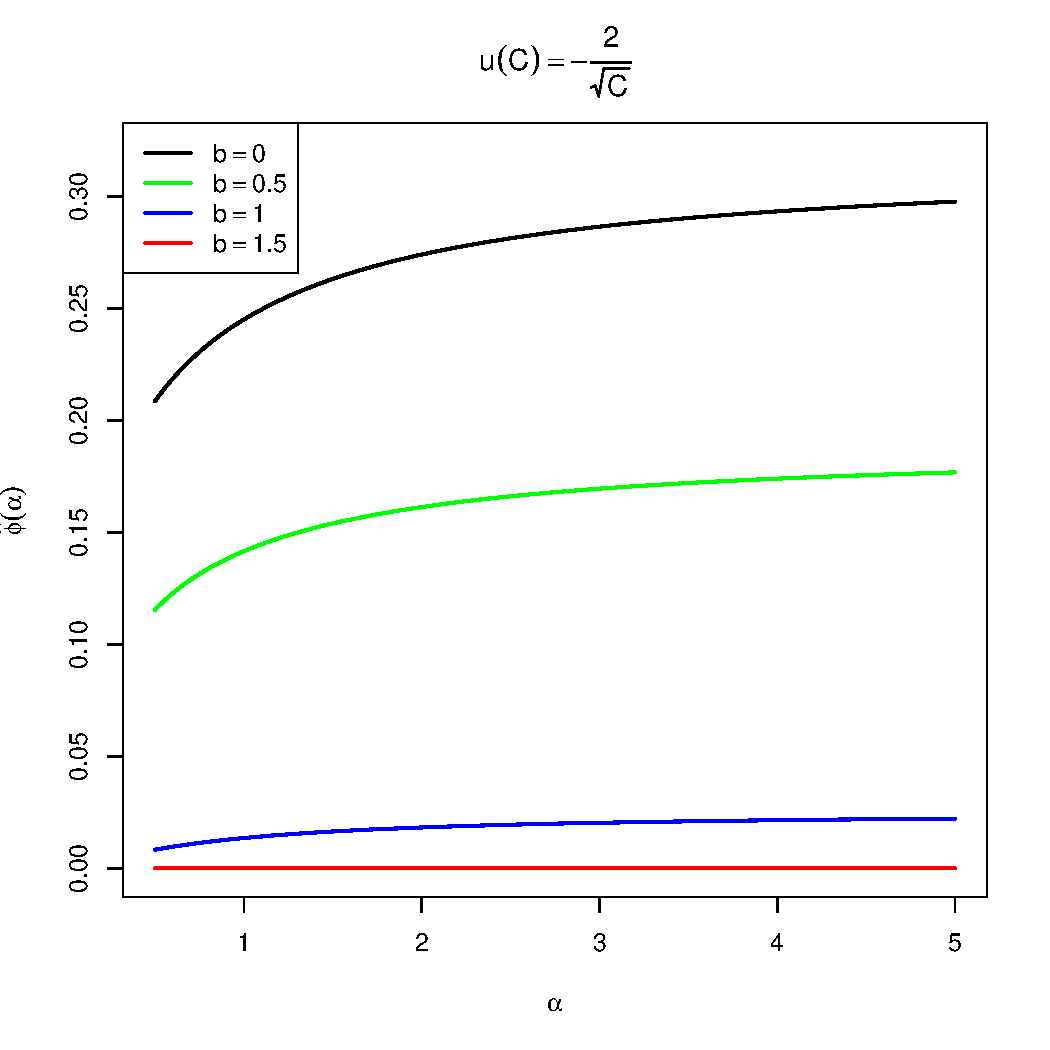
\includegraphics[width=\textwidth]{phi_hat_b_t_power.pdf}
  \end{minipage}\hfill
  \begin{minipage}{0.5\linewidth}
    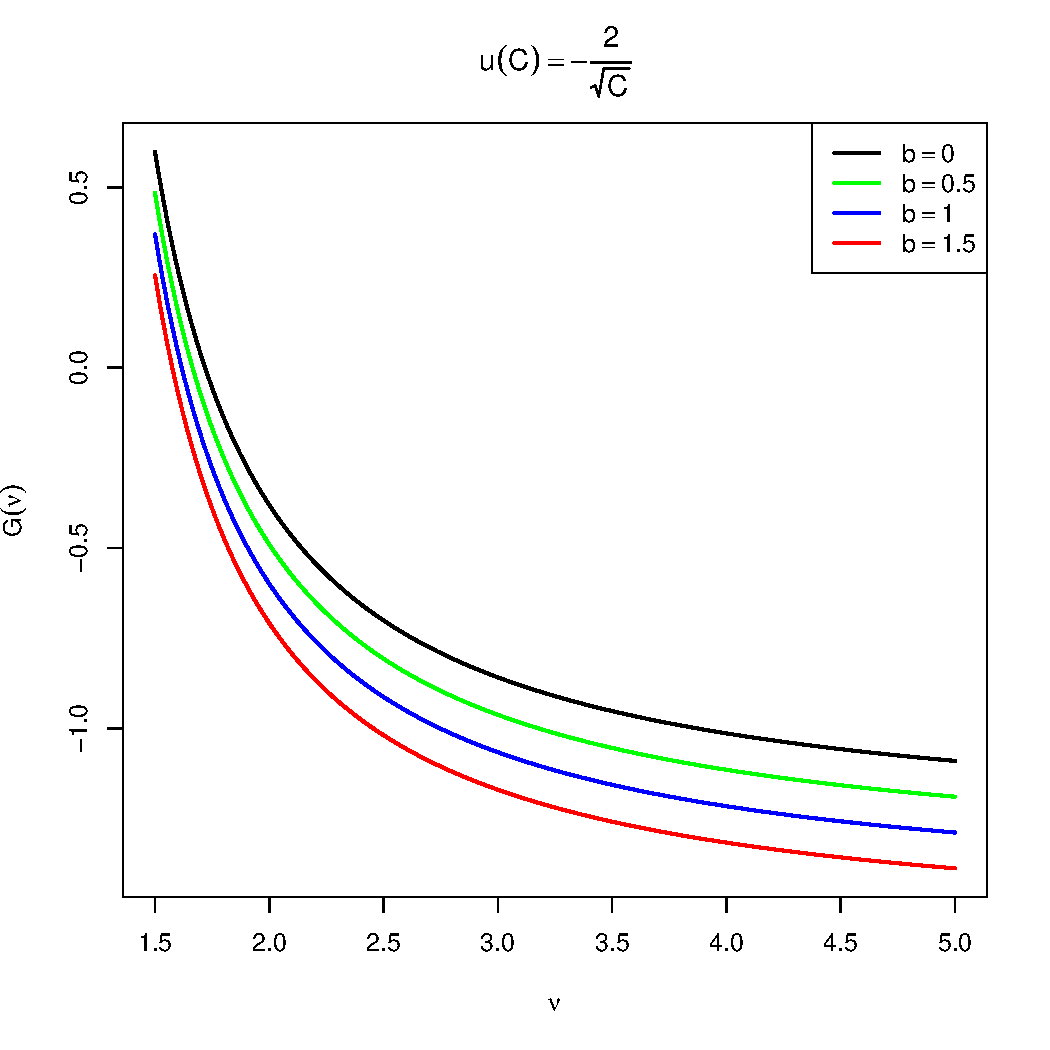
\includegraphics[width=\textwidth]{U_b_t_power.pdf}
  \end{minipage}
  \begin{minipage}{0.5\linewidth}
    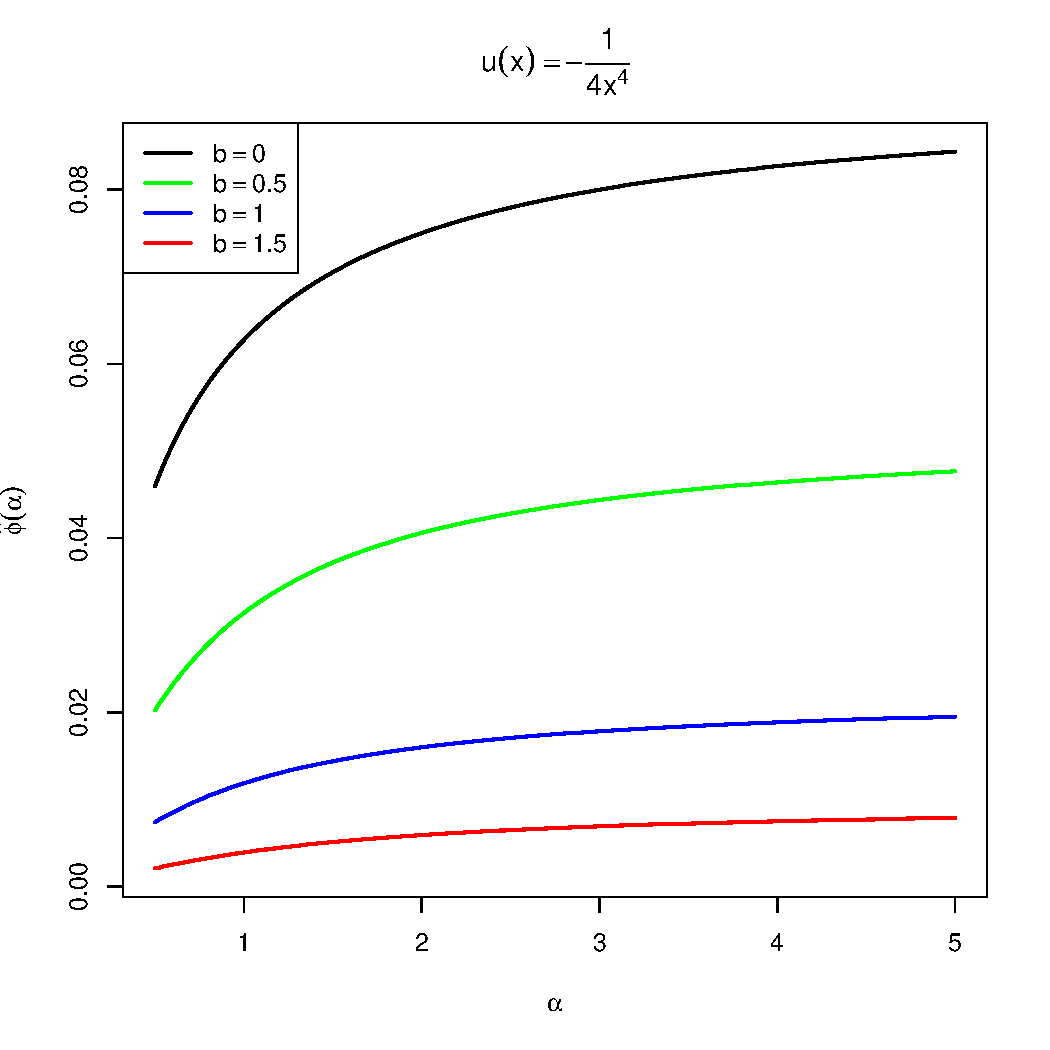
\includegraphics[width=\textwidth]{phi_hat_b_t_power4.pdf}
  \end{minipage}\hfill
  \begin{minipage}{0.5\linewidth}
    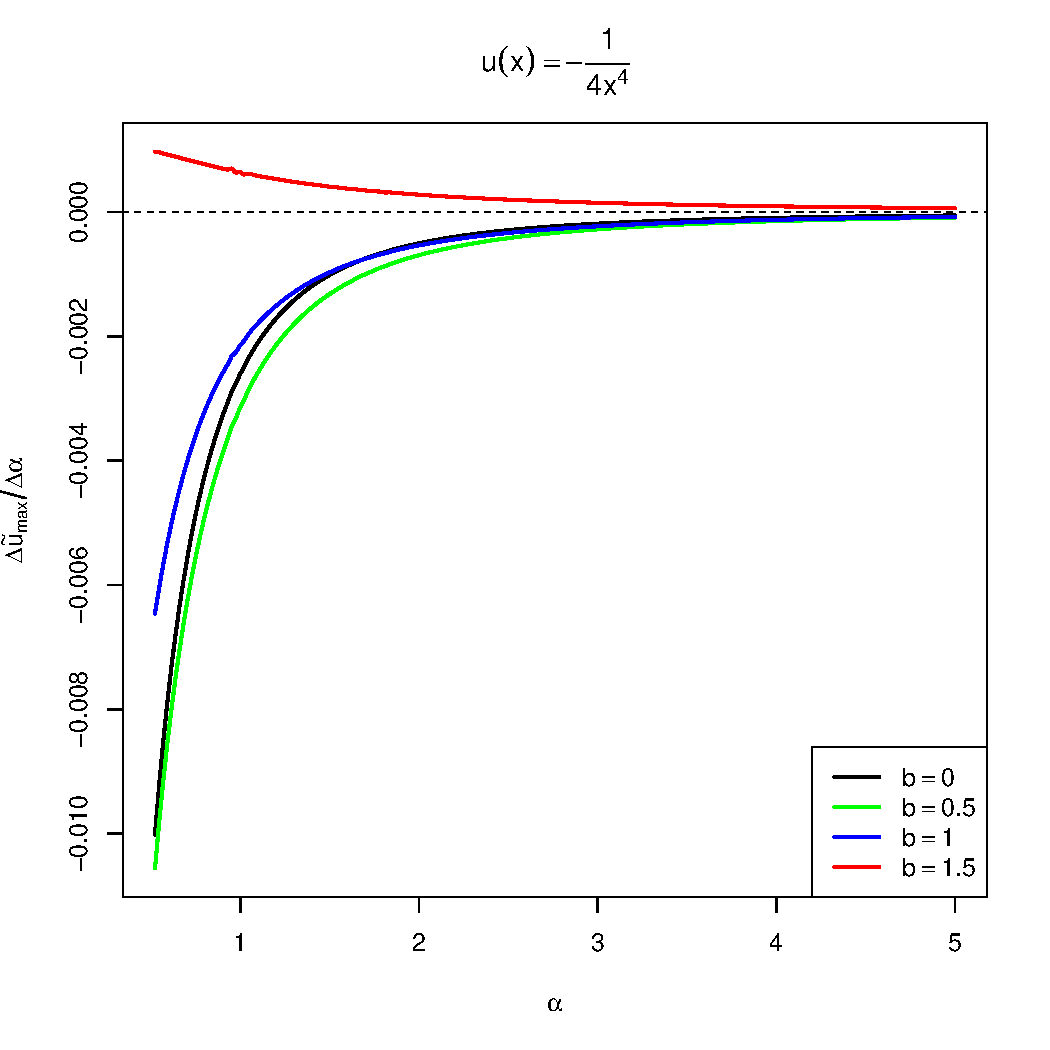
\includegraphics[width=\textwidth]{U_b_t_power4.pdf}
  \end{minipage}
  \caption{$\hat\phi$ (left) and ${\pd \tilde u_{\rm max} \over \pd
      \alpha}$ (right). {\em top:} $\xi = 1/2$. {\em bottom:} $\xi =
    4$.
  }
  \label{fig:htfg}
\end{figure}
\begin{lemma}
  \label{lemma:II}
  Let $f$ denotes the density function of the Student's
  t-distribution, i.e.
  \[
  f(x; \alpha) = c(\alpha) \left(
    1 + {x^2 \over \alpha}
  \right)^{-(\alpha + 1)/2}
  \]
  where $\alpha > 1$ and
  \[
  c(\alpha) = {
    \Gamma({\alpha + 1 \over 2})
    \over
    \Gamma(\alpha/2) \sqrt{\alpha \pi}
  }
  \]
  Then there exists $x_0 > 0$ such that ${\pd f \over
    \pd \alpha}(x_0, \alpha) = 0$ and $\forall x \in (0, x_0), {\pd f \over
    \pd \alpha}(x, \alpha) > 0$ and $\forall x \in (x_0, \infty), {\pd f
    \over \pd \alpha}(x, \alpha) < 0$.
\end{lemma}
\begin{proof}
  Straightforward computation gives
  \begin{eqnarray}
    {\pd f(x, \alpha) \over \pd \alpha} &=& {
      c(\alpha) x^2 (\alpha + 1) + (2 \alpha x^2 + 2 \alpha^2) c'(\alpha)
      -
      \alpha c(\alpha) (x^2 + \alpha) \log(1 + x^2/\alpha)
      \over
      2 \alpha (x^2 + \alpha) (1 + x^2 / \alpha)^{\alpha/2 + 1/2}
    } \nonumber \\
    &:=& {
      P(x^2, \alpha)
      \over
      2 \alpha (x^2 + \alpha) (1 + x^2 / \alpha)^{\alpha/2 + 1/2}
    }
    \label{eq:xxie4.1}
  \end{eqnarray}

  While the denominator of the right side of ${\pd f(x, \alpha) \over \pd \alpha}$ is
  always positive, its numerator $P(x^2, \alpha)$ has a single root:
  \begin{equation}
    \label{eq:xxie5}
    x_0^2 = \alpha\exp\left\{
      W\left[
        -\left(1 + {1 \over \alpha}\right)
        e^{-1 - 2 c'(\alpha)/c(\alpha) - 1/\alpha}
      \right]
      + 1 + {1 \over \alpha} + {2 c'(\alpha) \over c(\alpha)}
    \right\} - \alpha
  \end{equation}
  where $W(\cdot)$ is the principle branch of the Lambert $W$
  function. and $c'(\cdot)$ is the derivative of $c(\cdot)$. To check
  the right side of \eqref{eq:xxie5} for positivity, we first note
  $c'(\alpha) > 0$:
  \[
  c'(\alpha) = {
    \pi \Gamma(\alpha/2 + 1/2) \left\{
      \alpha \left[ \Psi(\alpha/2 + 1/2) - \Psi(\alpha/2)\right] - 1
    \right\}
    \over
    2 \Gamma(\alpha/2) (\pi \alpha)^{3/2}
  }
  \]
  where $\Psi(\cdot)$ is the digamma function:
  \[
  \Psi(x) = {d \log[\Gamma(x)] \over d x}
  \]
  \begin{minipage}{0.48\textwidth}
    $\Psi(x)$ \linebreak
    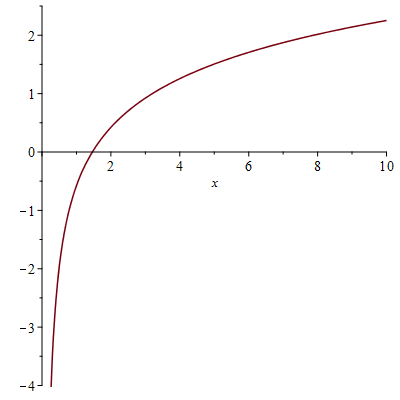
\includegraphics[width=\textwidth]{digamma.png}
  \end{minipage}\hfill
  \begin{minipage}{0.5\textwidth}
    As shown in the figure to the left, $\Psi(x)$ is increasing
    for $x > 0$. This immediately follows from the series
    representation
    \[
    \Psi(x + 1) = -\gamma + \sum_{n=1}^\infty {x \over n(n + x)}
    \quad x \neq -1, -2, -3,\dots
    \]
    which gives
    \[
    {\pd \Psi(x + 1) \over \pd x}
    = \sum_{n=1}^\infty {1 \over (n + x)^2} > 0
    \]
    See Abramowitz and Stegun \cite{abramowitz1972handbook}, p.259,
    formula 6.3.16. Therefore $\Psi(\alpha/2 + 1/2) - \Psi(\alpha/2) > 0$.
    So we have
    \begin{eqnarray*}
      && \alpha \left[
        \Psi(\alpha/2 + 1/2) - \Psi(\alpha/2)
      \right] - 1 \\
      &\geq& 1 \times \left[
        \Psi(1/2 + 1/2) - \Psi(1/2)
      \right] - 1 \\
      &=& \log(4) - \log(e) \\
      &>& 0
    \end{eqnarray*}
    Thus $c'(\alpha) > 0$. Furthermore, we recall
    $W(\cdot)$ is increasing on its principle branch. So
  \end{minipage}
  \begin{eqnarray*}
    &&
    W\left[
      -\left( 1 + {1 \over \alpha} \right)
      e^{-1 - 2 c'(\alpha)/c(\alpha) - 1/\alpha}
    \right]
    + 1 + {1 \over \alpha} + {2 c'(\alpha) \over c(\alpha)} \\
    &>& 
    W\left[
      -\left( 1 + {1 \over \alpha} + {2 c'(\alpha) \over c(\alpha)} \right)
      e^{-1 - 2 c'(\alpha)/c(\alpha) - 1/\alpha}
    \right]
    + 1 + {1 \over \alpha} + {2 c'(\alpha) \over c(\alpha)} \\
    &=& W(-y e^{-y}) + y
  \end{eqnarray*}
  where
  \[
  y = 1 + {1 \over \alpha} + {2 c'(\alpha) \over c(\alpha)} > 1
  \]
  Now notice
  \[
  \log(y e^{-y}) = \log(y) - y
  \]
  is a decreasing function for $y > 1$. Thus $-y e^{-y}$ is an
  increasing function. Hence we have
  \begin{eqnarray*}
    W(-y e^{-y}) + y &>& W(-e^{-1}) + 1 = 0
  \end{eqnarray*}
  Now it is clear
  \[
  \alpha\exp\left\{
    W\left[
      -\left(1 + {1 \over \alpha}\right)
      e^{-1 - 2 c'(\alpha)/c(\alpha) - 1/\alpha}
    \right]
    + 1 + {1 \over \alpha} + {2 c'(\alpha) \over c(\alpha)}
  \right\} - \alpha > 0
  \]
  Now that we have established that ${\pd f \over \pd \alpha}(x,
  \alpha) = 0$ has a single positive root, it remains to determine the
  sign of ${\pd f \over \pd \alpha}(x, \alpha)$ on the two sides of
  the root. For this purpose we observe
  \begin{equation}
    \label{eq:xxie5.1}
    P(0, \alpha) = 2 \alpha^2 c'(\alpha) > 0
  \end{equation}
  So we want to investigate ${\pd P \over \pd x}(x, \alpha)$:
  \begin{eqnarray}
    {\pd P \over \pd x}(x, \alpha) &=&
    2 \alpha c'(\alpha) + c(\alpha) - \alpha c(\alpha) \log\left(
      1 + {x \over \alpha}
    \right)
    \label{eq:xxie6}
  \end{eqnarray}
  Clearly, $\frac{\pd P}{\pd x}(0, \alpha) > 0$. Hence from
  \eqref{eq:xxie5.1} and
  \eqref{eq:xxie6} it is clear
  \begin{equation*}
    \text{sign}\left[
      {\pd f \over \pd\alpha}(x, \alpha)
    \right]
    = \left\{
    \begin{array}{rl}
      1 & 0 < x < x_0 \\
      -1 & x > x_0
    \end{array}
    \right.
  \end{equation*}
  where $x_0$ is the positive root of \eqref{eq:xxie5}.
\end{proof}

\section{Proof of Lemma~\ref{thrm:I}}
\setcounter{equation}{0}
\label{sec:thrmI_proof}
\begin{proof}
  Let
  \begin{equation}
    \label{eq:xxie2}
    \hat \phi := \underset{0 < \phi \leq 1}{\text{argmax}}\,
    \wt u(F_X, \phi)
  \end{equation}
  We have
  \[
  \tilde u_{\rm max}(F_X) = \wt u(F_X, \hat\phi)
  \]
  It follows
  \begin{eqnarray}
    {d \tilde u_{\rm max}(F_X) \over d \alpha}
    &=&
    \left.{\pd \wt u(\alpha, \phi) \over \pd \alpha}\right|_{\phi = \hat\phi}
    + \left.{\pd \wt u(\alpha, \phi) \over \pd \phi}\right|_{\phi = \hat\phi}
    {\pd \hat\phi \over \pd \alpha}
    \label{eq:xxie3}
  \end{eqnarray}
  The definition \eqref{eq:xxie2} implies for all $\alpha$
  \begin{equation}
    \label{eq:xxie4}
    \left.{\pd \wt u(\alpha, \phi) \over \pd \phi}\right|_{\phi = \hat\phi} = 0
  \end{equation}
  So the second term of \eqref{eq:xxie3} vanishes. It remains to show
  the first term is positive. From \eqref{eq:xxie1.0}, it follows
  \begin{eqnarray*}
    {\pd \wt u(\alpha, \phi) \over \pd \alpha}
    = {\partial \over \partial \alpha}\E[u((1 - \phi) e^r + \phi e^x) \1_{\{X < 0\}}]
  \end{eqnarray*}
  The function $u((1 - \phi) e^r + \phi e^x)$ is obviously
  increasing with $x$. It follows
  \begin{eqnarray*}
    {\pd f_X(x; \alpha, K) \over \pd \alpha}
    = {\partial \over \partial \alpha} {\alpha K^\alpha \over (K - x)^{\alpha + 1}} 
    = - {K^\alpha \over (K - x)^{\alpha + 1}}
    \left[
      \alpha
      \log\left(
        1 - {x \over K}
      \right) - 1
    \right]
  \end{eqnarray*}
  It is easily checked
  \[
  {\partial \over \partial \alpha}
  {\alpha K^\alpha \over (K - x)^{\alpha + 1}}
  \left\{
    \begin{array}{ll}
      > 0 & \text{ when } x < K(1 - e^{1/\alpha}) < 0 \\
      < 0 & \text{ when } K(1 - e^{1/\alpha}) < x < 0
    \end{array}
  \right.
  \]
% that when $x < K(1 - e^{1/\alpha}) < 0$,
%   \[
%   {\partial \over \partial \alpha} {\alpha K^\alpha \over (K - x)^{\alpha + 1}} < 0
%   \]
%   and when $K(1 - e^{1/\alpha}) < x < 0$,
%   \[
%   {\partial \over \partial \alpha} {\alpha K^\alpha \over (K - x)^{\alpha + 1}} > 0
%   \]
  This is the second case of lemma \ref{lemma:I}. So we have
  ${\pd \wt u(\alpha, \phi) \over \pd \alpha} > 0$.
  As for ${\pd \tilde u_{\rm max}(F_X) \over \pd K}$, by the same
  argument, it suffices to show ${\pd \wt u(K, \phi) \over \pd K} < 0$.
  We have
  \[
  {\pd \wt u(K, \phi) \over \pd K}
  = {\partial \over \partial K} \E \left[
    u((1 - \phi) e^r + \phi e^x) \1_{\{X < 0\}}
  \right] 
  \]
  and
  \begin{eqnarray*}
    {\pd f_X(x; \alpha, K) \over \pd K}
    = {\partial \over \partial K} {\alpha K^\alpha \over (K - x)^{\alpha + 1}}
   = -\alpha K^{\alpha - 1} {
      \alpha x + K
      \over
      (K - x)^{\alpha + 2}
    }
  \end{eqnarray*}
  Clearly,
  \[
  {\partial \over \partial K}
  {\alpha K^\alpha \over (K - x)^{\alpha + 1}}
  \left\{
    \begin{array}{ll}
      > 0 & \text{ when } x < -K/\alpha < 0\\
      < 0 & \text{ when } -K/\alpha < x < 0
    \end{array}
  \right.
  \]
  % Clearly, when $x < -K/\alpha$
  % \[
  % {\partial \over \partial K} {\alpha K^\alpha \over (K - x)^{\alpha + 1}} > 0
  % \]
  % and when $-K/\alpha < x < 0$
  % \[
  % {\partial \over \partial K} {\alpha K^\alpha \over (K - x)^{\alpha + 1}} < 0
  % \]
  So by the 1st case of Remark \ref{remark:I} we conclude $  {\pd \wt u(K, \phi) \over \pd K} < 0$.
\end{proof}

\section{Lemma~\ref{lemma:III}}
\setcounter{equation}{0}
\begin{lemma}\label{lemma:III}
Let $u(\cdot)$  and $C(\cdot)$ be defined as in \eqref{eq:hjyr} and
\eqref{eq:xxie1} respectively. Define
\begin{eqnarray*}
U_{\text{all}} &=& u(C(x))
+ u(C(-x))
\quad
x \geq 0 \\
a &=& {
  (1 - \phi) e^r
  \over
  \phi
} \\
y_\pm &=& {
  a^2 - \xi \pm \sqrt{(a^2 - 1) (a^2 - \xi^2)}
  \over
  a (\xi - 1)
}
\end{eqnarray*}
The following holds true:
\begin{enumerate}
\item If $\max\{a, 1\} < \xi$, $U_{\text{all}}(\cdot)$ is
  monotone decreasing.
\item If $a < \xi < 1$ and $(a + y_-)/(a y_- + 1) <
  y_-^{(1-\xi)/(1+\xi)}$, $U_{\text{all}}(\cdot)$ is monotone
  decreasing.
\item If $\xi < a < 1$, $U_{\text{all}}(\cdot)$ is monotone
  increasing.
\item If $1 < \xi < a$ and $(a + y_+)/(a y_+ + 1) >
  y_+^{(1-\xi)/(1+\xi)}$, $U_{\text{all}}(\cdot)$ is monotone
  increasing.
\item In other case, $U_{\text{all}}(\cdot)$ is not monotone.
\end{enumerate}
\end{lemma}
\begin{proof}
  It is convenient to re-write $U_{\text{all}}$ as
  \[
  U_{\text{all}} =
  -{\phi^{-\xi} \over \xi} \left\{
    \underbrace{
      \left[{(1 - \phi) \over \phi} e^r + e^x\right]^{-\xi}
      +
      \left[{(1 - \phi) \over \phi} e^r + e^{-x}\right]^{-\xi}
    }_{U(x)}
  \right\}
  \]
  Thus the monotonicity of $U_{\text{all}}(x)$ is the opposite of $U(x)$. For
  convenience of writing, let $a = (1 - \phi)e^r/\phi$.
  First of all, we find the conditions on which $U(x)$ is monotone.
  Direct differentiation yields
  \begin{eqnarray*}
    {\pd U(x) \over \pd x}
    &=&
    -{
      (a + e^x)^{-\xi - 1} \xi e^x
    } + (a + e^{-x})^{-\xi - 1} \xi e^{-x}
  \end{eqnarray*}
  ${\pd U(x) \over \pd x} = 0$ is equivalent to
  \begin{eqnarray*}
    {a + y \over a y + 1} &=& y^{1 -\xi \over 1+\xi} \\
    \underbrace{\log(a + y) - \log(a y + 1)}_{f(y)} &=&
    {1 -\xi \over 1+\xi} \log(y)
  \end{eqnarray*}
  where we have defined $y = e^x$, and $f(y)$, $g(y)$ as above. Observe
  \begin{equation}
    \label{eq:f-g-der}
    {\pd (f -g)(y) \over \pd y} = {
      a (\xi - 1) y^2 + 2 (\xi - a^2) y + a(\xi - 1)
      \over
      (1 + \xi) (a + y) (a y + 1) y
    }
  \end{equation}
  ${\pd (f -g)(y) \over \pd y} = 0$ has two roots when $\xi \ne 1$
  \begin{eqnarray*}
    y_\pm &=& {
      a^2 - \xi \pm \sqrt{(a^2 - 1) (a^2 - \xi^2)}
      \over
      a (\xi - 1)
    }
  \end{eqnarray*}
  \begin{enumerate}
  \item If $\min\{1, \xi\} < a < \max\{1, \xi\}$, $y_\pm$ are not
    real, ${\pd (f -g)(y) \over \pd y} = 0$ has no solution on
    $(1, \infty)$; $(f -g)(y)$ is monotone on $(1, \infty)$.
    \begin{enumerate}
    \item If in addition $\xi > 1$, i.e. $1 < a < \xi$, $(f - g)(y)$
      is monotone increasing on $(1, \infty)$, because the
      coefficient of the $y^2$ term of the numerator of
      \eqref{eq:f-g-der}, i.e. $a (\xi - 1)$ is positive. We note
      $f(1) = g(1) = 0$; thus on $(1, \infty)$, there is no solution
      to $f(y) = g(y)$. It can be concluded that $U(\cdot)$ is
      monotone on $(0, \infty)$. Furthermore
        \begin{eqnarray*}
          \left.{\pd U(x) \over \pd x}\right|_{x=0} &=& 0 \\
        \end{eqnarray*}
        For a small $\epsilon > 0$, the sign of ${\pd U(x) \over \pd
          x}$ on $(0, \epsilon)$ is thus the same as
        $\left.{\pd^2 U(x) \over \pd x^2}\right|_{x=0}$:
        \[
        \left.{\pd^2 U(x) \over \pd x^2}\right|_{x=0} =
        2 (a + 1)^{-\xi - 2} (\xi - a) > 0
        \]
        Thus ${\pd U(x) \over \pd x} > 0$ for $x \in (0, \infty)$;
        $U_{\text{all}}$ is monotone decreasing.
    \item If instead $\xi < 1$, i.e. $\xi < a < 1$, by a similar
      argument as in the previous case, $U_{\text{all}}$ is monotone
      increasing on $(0, \infty)$.
    \end{enumerate}
  \item If $a < \min\{1, \xi\}$ and $\xi > 1$, i.e. $a < 1 < \xi$, it
    is clear
    \[
    y_- = {
      a^2 - \xi - \sqrt{(a^2 - 1) (a^2 - \xi^2)}
      \over
      a (\xi - 1)
    } < 0
    \]
    It remains to compare $y_+$ with $1$ to determine whether
    ${\pd (f -g)(y) \over \pd y} = 0$ has a solution on $(1, \infty)$.
    Assume $y_+ > 1$. Then
    \begin{eqnarray}
      a^2 - \xi + \sqrt{(a^2 - 1) (a^2 - \xi^2)} &>& a (\xi - 1)
      \nonumber \\
      2 a (\xi - 1) (a + 1) (a - \xi) &>& 0 \label{eq:mi6}
    \end{eqnarray}
    This contradicts the assumption $a < \xi$ and $\xi > 1$. Hence
    $y_+ < 1$. So we conclude $(f - g)(y)$ is monotone increasing
    on $(1, \infty)$. Following the same analysis as in the case
    (1.a), one can see $U_{\text{all}}$ is monotone decreasing.

  \item If $a < \min\{1, \xi\}$ and $\xi < 1$, i.e. $a < \xi < 1$, it
    is clear $y_- > 0$ and $y_+ < y_-$. Moreover, $y_- > 1$ is equivalent
    to
    \[
    \sqrt{(a^2 - 1) (a^2 - \xi^2)} > a^2 - \xi a + a - \xi
    = (a + 1) (a - \xi)
    \]
    The last inequality is obviously true in this case. So $y_- >
    1$. ${\pd (f-g)(y) \over \pd y}$ has a maximum at
    $y_- \in (1, \infty)$. We know $(f - g)(y_-)$ is a maximum because
    \eqref{eq:f-g-der} shows that, for $y > y_-$,
    ${\pd (f-g)(y) \over \pd y} < 0$.

    If $(f-g)(y_-) < 0$, $(f-g)(y) = 0$ has no solution on $(1,
    \infty)$. Hence $U(\cdot)$ is monotone on both $(0, \infty)$.
    The same analysis as in the case (1.a) shows $U_{\text{all}}$
    is monotone decreasing on $(0, \infty)$.

    If $(f-g)(y_-) > 0$, $(f-g)(y) = 0$ must have a solution on $(y_-,
    \infty)$. So $U(\cdot)$ is not monotone.

    \item $a > \max\{1, \xi\}$ and $\xi > 1$, i.e. $1 < \xi < a$. By
      the same argument that leads to \eqref{eq:mi6}, we see
      $y_+ > 1$. From \eqref{eq:f-g-der} it is clear $(f-g)(y_+)$ is a
      minimum. If $(f-g)(y_+) > 0$, there is no solution to
      $(f-g)(y) = 0$ on $(1, \infty)$; $U(x)$ is monotone. By the
      same analysis as in the case (1.a), we know $U(x)$ is
      monotone decreasing and $U_{\text{all}}$ is monotone increasing.
      
      if $(f-g)(y_+) < 0$, there must be a solution to $(f-g)(y) = 0$
      on $(y_+, \infty)$. $U_{\text{all}}$ is not monotone.
  \end{enumerate}
\end{proof}

\ifx\phdthesis\undefined
\else
\end{subappendices}
\fi
